\documentclass[10pt,twocolumn,letterpaper]{article}

\usepackage{cvm}
\usepackage{times}
\usepackage{epsfig}
\usepackage{graphicx}
\usepackage{amsmath}
\usepackage{amssymb}
\usepackage{subcaption}
\usepackage{multicol}
\usepackage{floatrow} 
%\usepackage[polish]{babel}
% Include other packages here, before hyperref.

% If you comment hyperref and then uncomment it, you should delete
% egpaper.aux before re-running latex.  (Or just hit 'q' on the first latex
% run, let it finish, and you should be clear).
\usepackage[pagebackref=true,breaklinks=true,letterpaper=true,colorlinks,bookmarks=false]{hyperref}


% \cvmfinalcopy % *** Uncomment this line for the final submission

\def\cvmPaperID{****} % *** Enter the cvm Paper ID here
\def\httilde{\mbox{\tt\raisebox{-.5ex}{\symbol{126}}}}

% Pages are numbered in submission mode, and unnumbered in camera-ready
\ifcvmfinal\pagestyle{empty}\fi
\begin{document}

%%%%%%%%% TITLE
\title{Efficient sketch-based character modelling with primitive deformer and shape generator}

\author{First Author\\
Institution1\\
Institution1 address\\
{\tt\small firstauthor@i1.org}
% For a paper whose authors are all at the same institution,
% omit the following lines up until the closing ``}''.
% Additional authors and addresses can be added with ``\and'',
% just like the second author.
% To save space, use either the email address or home page, not both
\and
Second Author\\
Institution2\\
First line of institution2 address\\
{\small\url{http://www.author.org/~second}}
}

\maketitle
% \thispagestyle{empty}

%%%%%%%%% ABSTRACT
\begin{abstract}
This paper proposes a new sketch-guided and ODE-driven character modelling technique. Our system consists of two main components: primitive deformer and detail generator. With such a technique, we first draw 2D silhouette contours of a character model. Then, we select proper primitives and align them with the corresponding silhouette contours. After that, we develop a sketch-guided and ODE-driven primitive deformer. It uses ODE-based deformations to deform the primitives to exactly match the generated 2D silhouette contours in one view plane and obtain a base mesh of a character model consisting of deformed primitives. In order to add various 3D details, we develop a local shape generator which uses sketches in different view planes to define a local shape and employs ODE-driven deformations to create a local surface passing through all the sketches.\\
The experimental results demonstrate that our proposed approach can create 3D character models with 3D details from 2D sketches easily, quickly and precisely.
\end{abstract}

%%%%%%%%% BODY TEXT
\section{Introduction}
\begin{itemize}
  \item[$\bullet$] We develop an efficient sketch-guided and ODE-driven primitive deformer to create a base mesh. It can deform primitives to exactly match the generated silhouette contours. Compared to the existing methods, it automates shape manipulation, avoids tedious manual operations, can deform primitives to match the generated silhouette contours quickly, and is powerful in achieving different shapes of a same primitive.
  \item[$\bullet$] We develop a detail generator to add 3D details to the base mesh. Our proposed sketch-guided and ODE-driven local shape creator can create a new local shape to match user's drawn sketches in different views quickly. The image-based detail generator can automatically generate fine details from 2D images. 
  \item[$\bullet$] Our character modelling system provide editing operations, support users to manipulate the control curves the draw in the creation stage and adding more control curves after the surface has been created. With our developed system, 3D character models with 3D details can be created easily and efficiently.
\end{itemize}
The rest of the paper is organised as follows. The previous related work is briefly reviewed in Section \ref{related_work}. The system overview of our proposed approach is presented in Section \ref{system_overview}. Primitive deformer is examined in Section \ref{primitive_deformer}, and Detail generator is investigated in Section \ref{detail_generator}. Finally, the conclusions and future work are discussed in Section \ref{conclusions_and_future_work}. 
\section{Related Work}\label{related_work}
\subsection{Inflation Technology}
Over the past two decades, sketch-based-modelling (SBM) has been widely studied in the computer graphic research community. Several research based systems have been proposed to generate organic models. The surface inflation technique extrudes the polygonal mesh from the skeleton outwards do a good job in modelling stuffed toys. One trend is to inflate freeform surfaces to create simple stuffed animals and other rotund objects in a sketch-based modelling fashion, such as \cite{igarashi1999teddy, Karpenko:2006:SFS:1141911.1141928, nealen2007fibermesh}. The Teddy system \cite{igarashi1999teddy} is the pioneer, it takes closed curves as inputs and find their cordial axes as spline, then wrap the splines with the polygonal mesh. Later, FiberMesh\cite{nealen2007fibermesh} enriched the editing operations for the inflating base mesh. FiberMesh also presents two types of the control curves: smooth and sharp. A smooth curve constrains the surface to be smooth across it, while a sharp curve only places positional constraints with C0 continuity. Sharp control curves appears when operations like cutting, extrusion and tunnel take place. Sharp control curves also serves the creation of creases on surface. However, FiberMesh \cite{nealen2007fibermesh} doesn't allow users to specify the ROI.Based on the study from William\cite{williams1997stochastic}, the SmoothSketch system addressed the problem of T-junction and cusp, which Teddy fails to solve.
%-------------------------------------------------------------------------
\subsection{Primitive Technology}
Unlike the inflating systems, primitives-based systems deconstruct the modelling task as a process of creating a certain set of geometry primitives and further editing on the primitives. The idea of assembling simple geometry primitives to form 3D models is very common in CSG(constructive solid geometry) modelling, related researches including \cite{shtof2013geosemantic,chen20133}. Shtof et.al \cite{shtof2013geosemantic} introduces a snapping method which helps determining the position and core parameters of several simple geometry primitives. In \cite{chen20133}, the authors provides tools for generating a cylinder from only 3 strokes: the first two strokes define the 2D profile and the last stroke defines the axis along which the profile curve will sweep. Copies of the profile are not only perpendicularly aligned to the axis, but also resized to snap to the input outlines. However their work is only for man-made objects which simple sweeping surface can meet the quality requirements of the shapes. Structured Annotations for 2D-to-3D Modelling \cite{gingold2009structured}, on the other hand, focus on organic modelling. It is a system using two sets of the primitives, one is generalized cylinders, created by the input of a single open sketch stroke representing the spline, and then modified by using simple gestures such as tilt, scale local radius, rotate symmetrical plane, and change cap size; the other primitive is ellipsoid, generated according to the drawn closed ellipse sketch stroke. As the system's name indicates, there are a set pf annotation tools to further editing the surface shape using the annotations such as same-lengths, same angles, alignment and mirror symmetry. 

\subsection{Mesh editing}
A universal disadvantage of above systems is features provided are limited it was not suited to modelling complex and production ready models. This is partly due to their limitations in mesh editing operations, so several sketch-based editing methods have been development to help to improve the performance of sketch-based modelling system. One group of sketch-based editing methods \cite{draper2003gestural, kho2005sketching} treats individual sketch curve as the reference for deformations like bending. Take the \cite{kho2005sketching} for example, user will draw a first curve as a reference curve to both set the ROI (region of interest) and be a controlling 'skeleton', and a new sketch curve indicating the desired deformation of the reference curve. Then mapping the reference curve to the second curve, the ROI will be deformed. These methods are very useful for simple keyframe animation, but for more small-scaled shape's editing task, studies like \cite{lipman2004differential,nealen2007sketch,SBM:SBM07:023-030} are more suitable. These studies take mesh's contours (depend on the viewplan at the time of editing operation is happening) as reference curves, and the newly sketched curves indicating the new positions that the ROI of mesh should be reconstructed to. As they aiming at maintaining the local geometrical details, Laplacian coordinates and correspondingly laplacian surface editing technology are implemented to preserving the features. 

\section{System Overview}\label{system_overview}
Based on our proposed approach, we have developed a modelling system which is composed of two main components: primitive deformer and detail generator. The primitive deformer is used to deform primitives to exactly match user's generated 2D silhouette contours and create a rough base mesh. The detail generator consists of local shape creator and image-based detail generator. The local shape creator creates a new local shape from four different algorithms. They are local shape creation from: 1) two open silhouette contours in two different view planes, 2) one open and one closed silhouette contour in two different view planes, 3) two open and one closed silhouette contours in three different view planes, and 4) two closed curves. The image-based detail generator generates fine 3D details from 2D images automatically through the SFS algorithm. \\
The modeling process using our developed system is demonstrated in Figure \ref{fig:system_overview} where a 3D female warrior model is created. \\
 \begin{figure}[h]
\begin{center}
%\fbox{\rule{0pt}{2in} \rule{0.9\linewidth}{0pt}}
 %  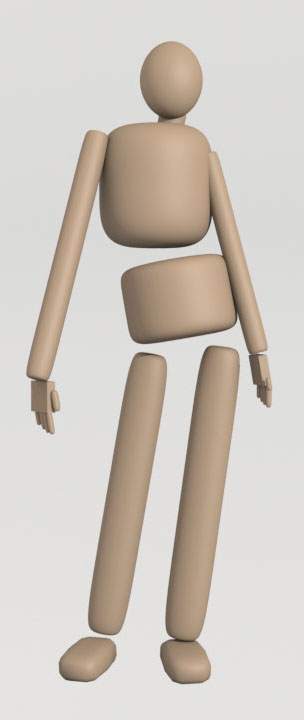
\includegraphics[width=0.7\linewidth]{./figure/primitives_before_deformation.jpg}\label{fig:long}
  \begin{subfigure}[t]{0.32\linewidth}
       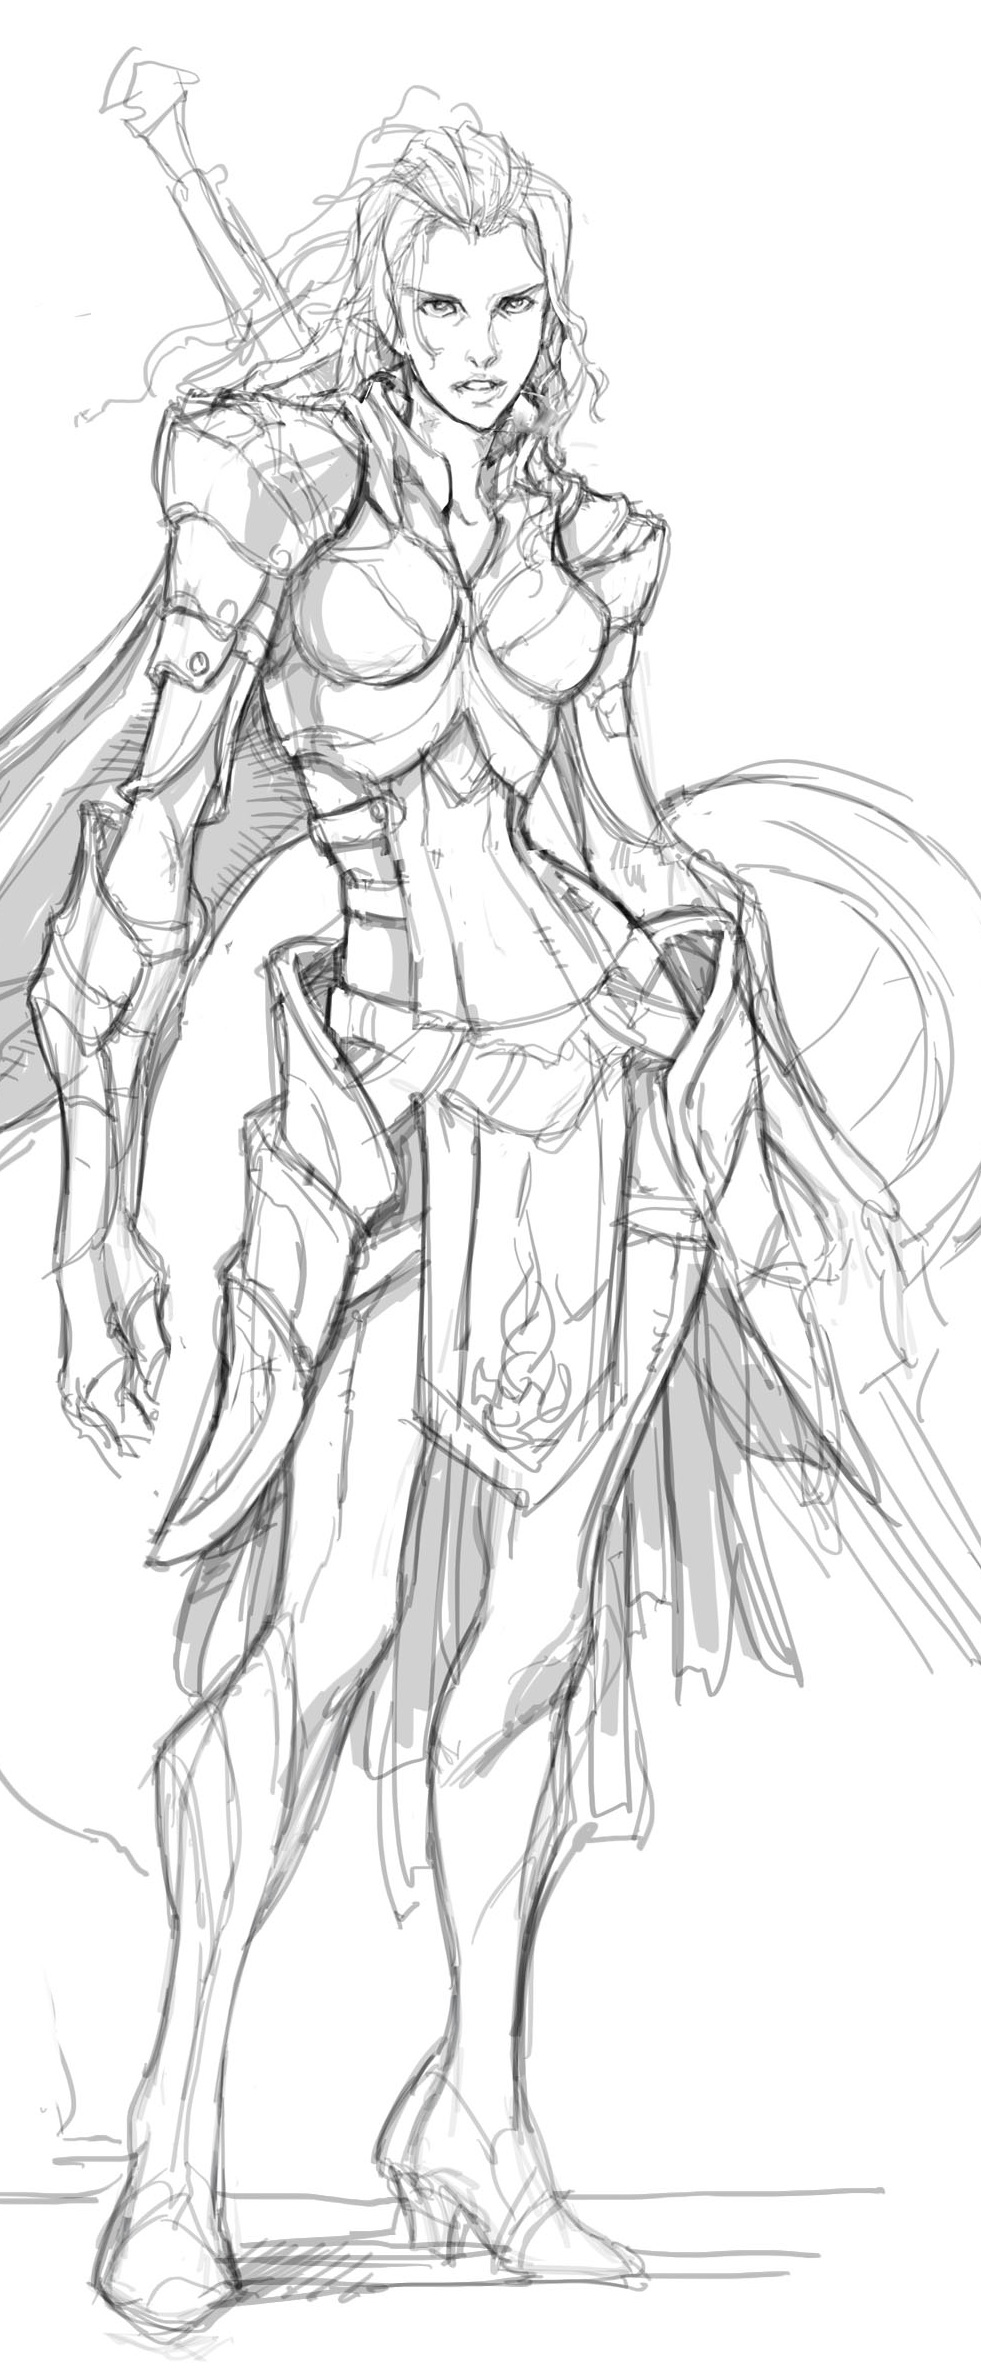
\includegraphics[height=2.3in]{./figure/female_warrior_original_sketch.jpg}
        \caption{}\label{fig:reference_image}
   \end{subfigure}
   \begin{subfigure}[t]{0.32\linewidth}
       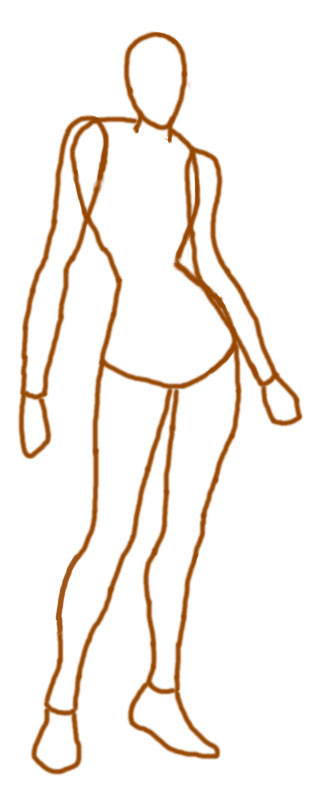
\includegraphics[height=2.3in]{./figure/female_warrior_extract_contour.jpg}
        \caption{}\label{fig:extract_contour}
   \end{subfigure}
 \begin{subfigure}[t]{0.32\linewidth}
       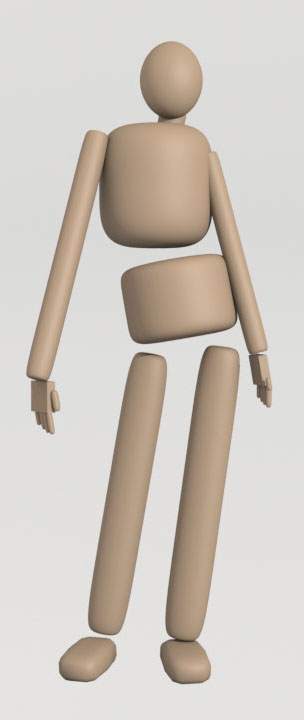
\includegraphics[height=2.3in]{./figure/primitives_before_deformation.jpg}
        \caption{}\label{fig:superellipsoid_primitives}
    \end{subfigure}
   % \hskip0.5em
    \begin{subfigure}[t]{0.32\linewidth}
        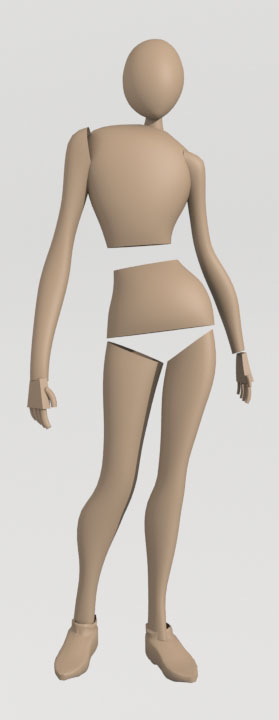
\includegraphics[height=2.3in]{./figure/primitives_after_deformation_without_blending.jpg}
        \caption{}\label{fig:primitives_after_deformation}
    \end{subfigure}
    \begin{subfigure}[t]{0.32\linewidth}
        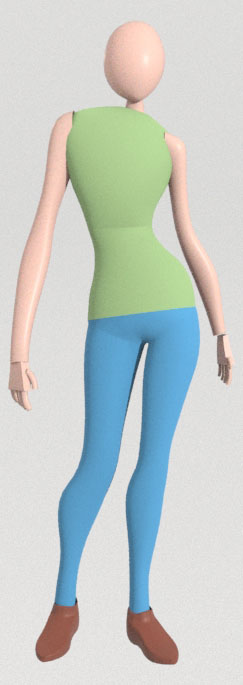
\includegraphics[height=2.3in]{./figure/primitives_after_deformation_and_lattice.jpg}
        \caption{}\label{fig:blending_body_parts}
    \end{subfigure}
    \begin{subfigure}[t]{0.32\linewidth}
        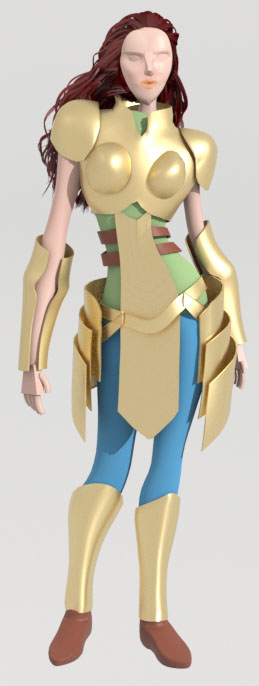
\includegraphics[height=2.3in]{./figure/final_shot.jpg}
        \caption{}\label{fig:final_shot}
    \end{subfigure}
\end{center}
   \caption{Quick creation of a 3D female warrior model: (a) 2D female warrior sketch, (b) 2D silhouette contours, (c) base mesh without primitive deformations, (d) base mesh by deforming primitives to match generated 2D silhouette contours or adding local shapes created from 2D silhouette contours, (e) base mesh by adding blending surfaces to smoothly connect deformed primitives, (f) detail generation through local shape creation and shape from shading (Sketch by � EngKit Leong)}
\label{fig:system_overview}
\end{figure}\\
First, 2D character silhouette contours are generated. Users can draw their own silhouette contours directly or input their selected sketches into our developed system. If the selected sketches are input into our developed system, a further process may be required to extract the 2D silhouette contours from the input sketches. For the example demonstrated in Figure \ref{fig:system_overview}, a 2D female warrior sketch shown in Figure \ref{fig:system_overview}\subref{fig:reference_image} is input. Then, users can extract 2D silhouette contours from the input sketch as shown in Figure \ref{fig:system_overview}\subref{fig:extract_contour}. After that, proper primitives are selected and placed to align with the corresponding silhouette contours through purely geometric transformations as shown in Figure \ref{fig:system_overview}\subref{fig:superellipsoid_primitives}. Since the silhouette contours of the primitives do not match the generated 2D silhouette contours of the 2D female warrior, the primitive deformer developed from sketch-guided and ODE driven deformations described in Section 4 is applied to deform the primitives to exactly match the corresponding 2D silhouette contours and create a rough 3D base mesh depicted in Figure \ref{fig:system_overview}\subref{fig:primitives_after_deformation}. \\
Once a 3D base mesh model is obtained, the detail generator described in Section 5 is employed to add 3D details to the 3D base mesh. First, the local shape creator developed in Subsection 5.2 is used to add local shapes and smoothly connect primitives together as demonstrated in Figure \ref{fig:system_overview}\subref{fig:blending_body_parts}. After that, we want to add fine details such as a dragon to the female warrior model. Since creating fine 3D details is not an easy task, we apply the image-based detail generator described in Subsection 5.3 to achieve the complicated 3D details shown in Figure \ref{fig:system_overview}\subref{fig:final_shot}.\\
In the following two sections, we will introduce in detail the primitive deformer and the detail generator, respectively. Some examples will be presented to demonstrate their applications.
\section{Primitive deformer}\label{primitive_deformer}
As shown in Figure \ref{fig:system_overview}\subref{fig:superellipsoid_primitives}, the base mesh of the female warrior without primitive deformations cannot exactly match the generated 2D silhouette contours of the female warrior. In order to tackle this problem, in this section, we develop a primitive deformer. In the subsections below, we first introduce the interface of the primitive deformer in Subsection \ref{user_interface_of_primitive_deformer}. Then, we discuss the algorithm of the primitive deformer in Subsection \label{algorithm_of_primitive_deformer}.
%------------------------------------------------------------------------
\subsection{User interface of primitive deformer}\label{user_interface_of_primitive_deformer}
The user interface of our developed primitive deformer uses four windows. The upper left window is used to display 3D base mesh without primitive deformations in the front view. The upper right window is used to display primitives and the user-drawn 2D silhouette contours for these primitives. If required, the user can edit the generated 2D silhouette contours in the upper right window. The deformed primitives are shown in the bottom windows where the left is from the front view and the right is from the side view. \\
Taking the left leg of the female warrior shown in Figure \ref{fig:deformer_UI} as an example, the primitive of the left leg is shown in the upper left window. It and the user-drawn 2D silhouette contours are depicted in the upper right window. Our proposed primitive deformer described in Subsection \ref{algorithm_of_primitive_deformer} deforms the primitives of the 3D base mesh to exactly match the generated 2D silhouette contours and create a deformed 3D base mesh with primitive deformations, and depicted the deformed 3D base mesh in bottom windows. \\
\begin{figure}[h]
\centering
       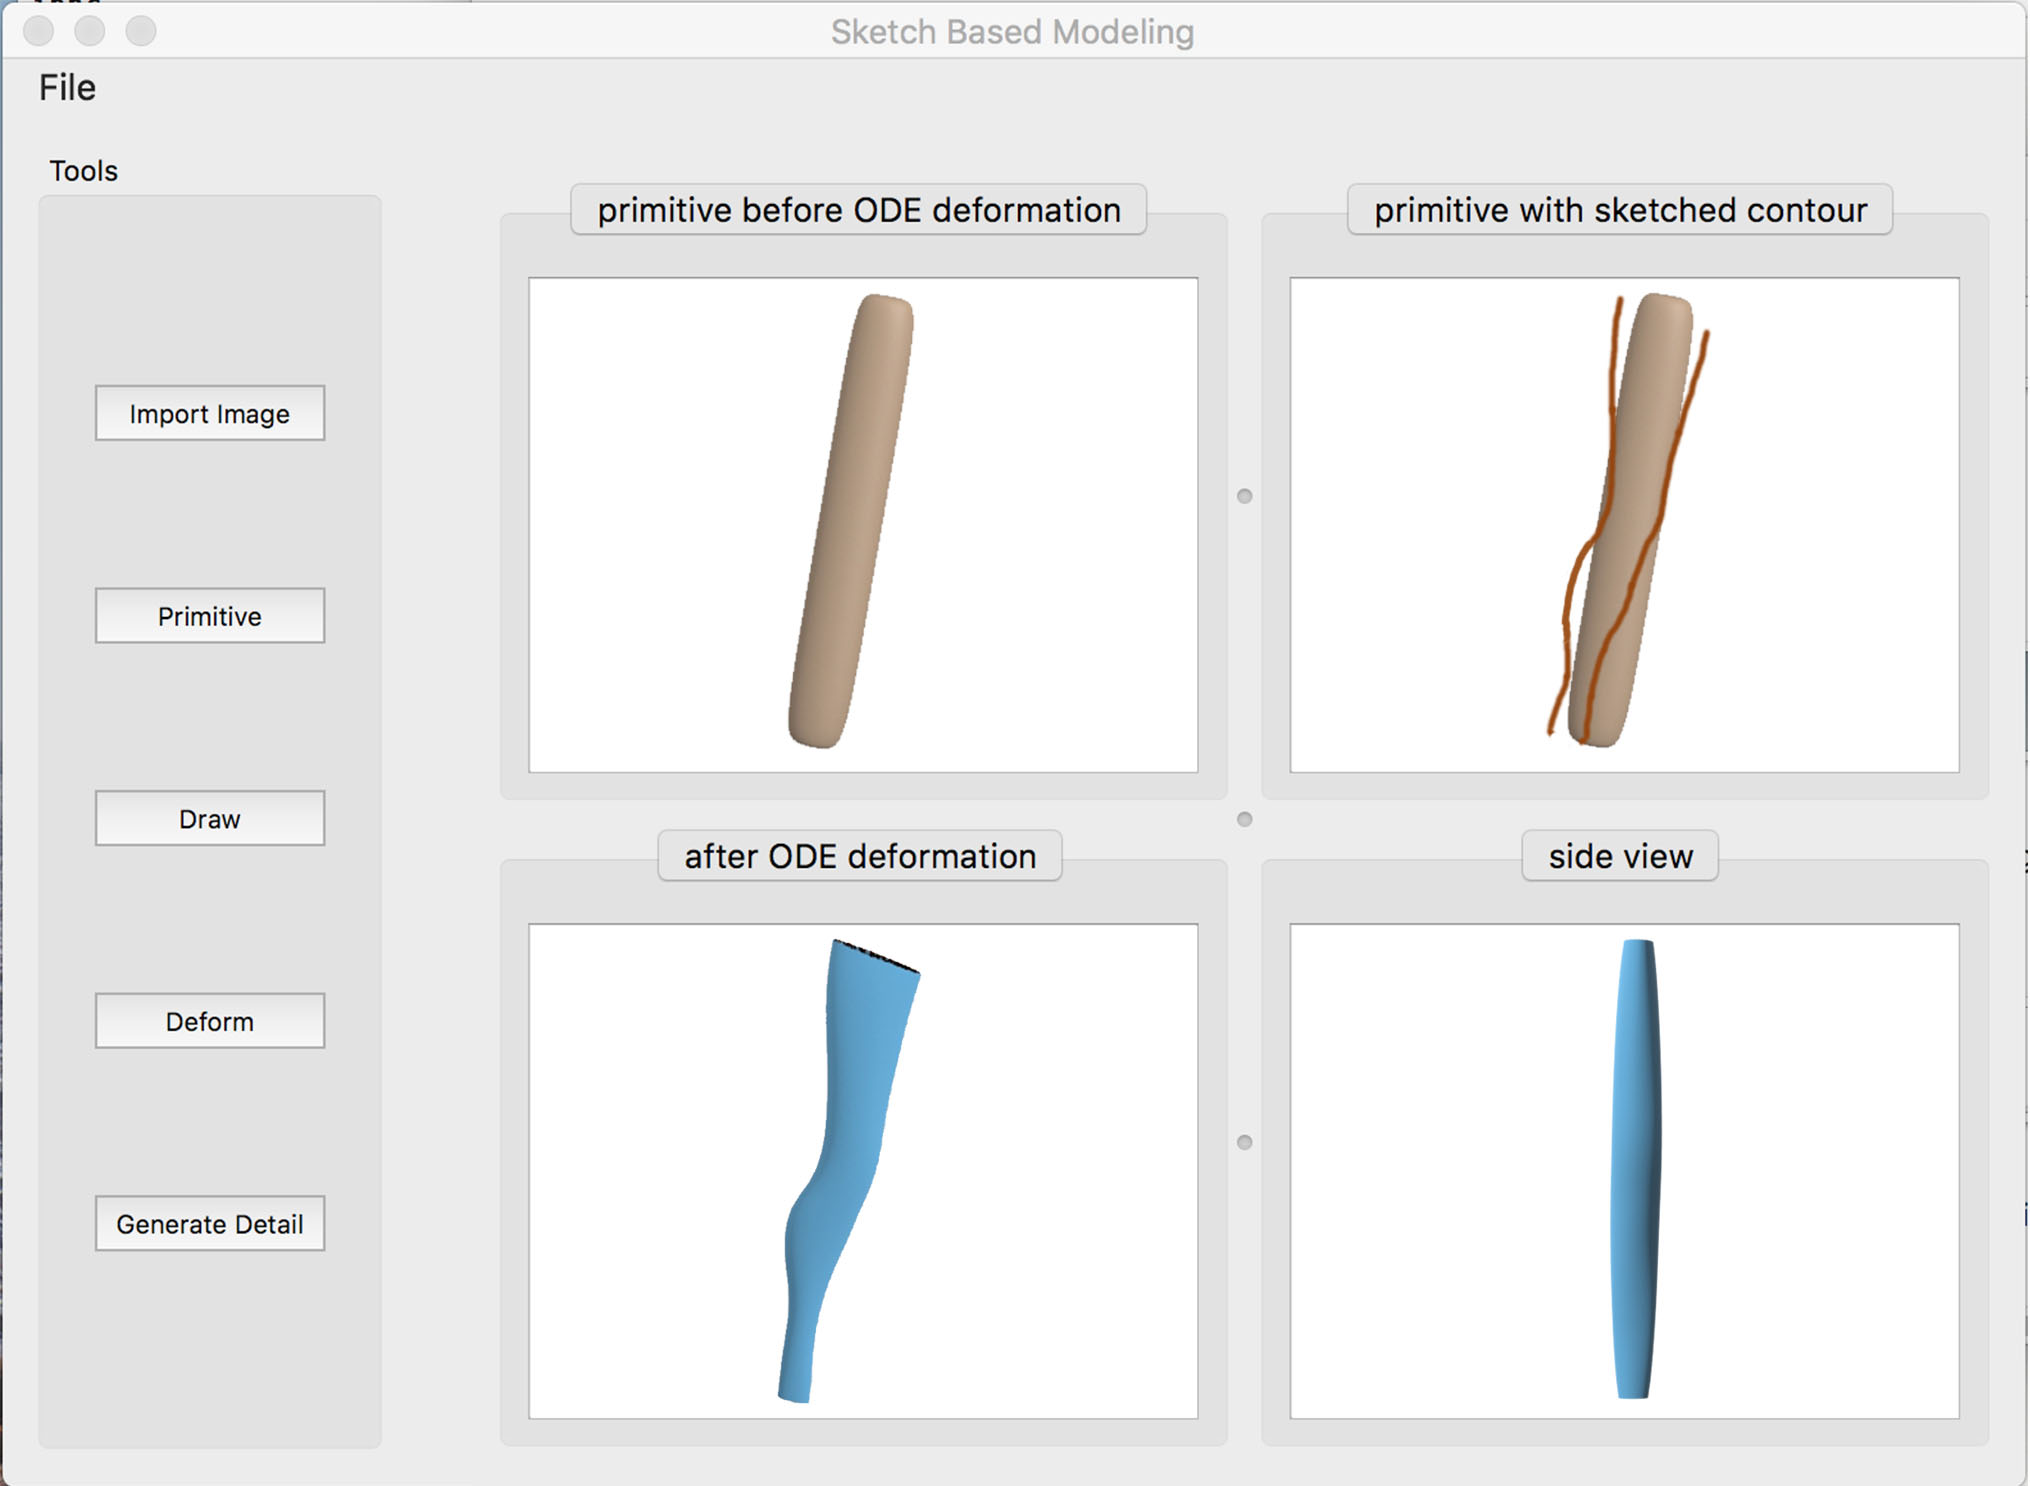
\includegraphics[width=1.0\linewidth]{./figure/deformer_UI.jpg}
\caption{Interface for primitive deformer: (a) 3D base mesh of the left leg of the female warrior without primitive deformations, (b) 2D silhouette contours of the female warrior leg sketch and primitive, (c) and (d) front view and side view of the 3D left leg base mesh after primitive deformations}
 \label{fig:deformer_UI}
\end{figure}
\subsection{Algorithm of primitive deformer}\label{algorithm_of_primitive_deformer}
After 3D primitives have been placed and aligned with the generated 2D silhouette contours, these 3D primitives should be deformed so that their 2D silhouette contours can match the generated 2D silhouette contours exactly. Here we use the example shown in Figure \ref{fig:torso} to demonstrate the algorithm of our proposed primitive deformer and how it deforms a 3D primitive to match the 2D silhouette contours. 
\begin{figure}[h]
\centering
 \begin{subfigure}[t]{0.45\linewidth}
 \centering
       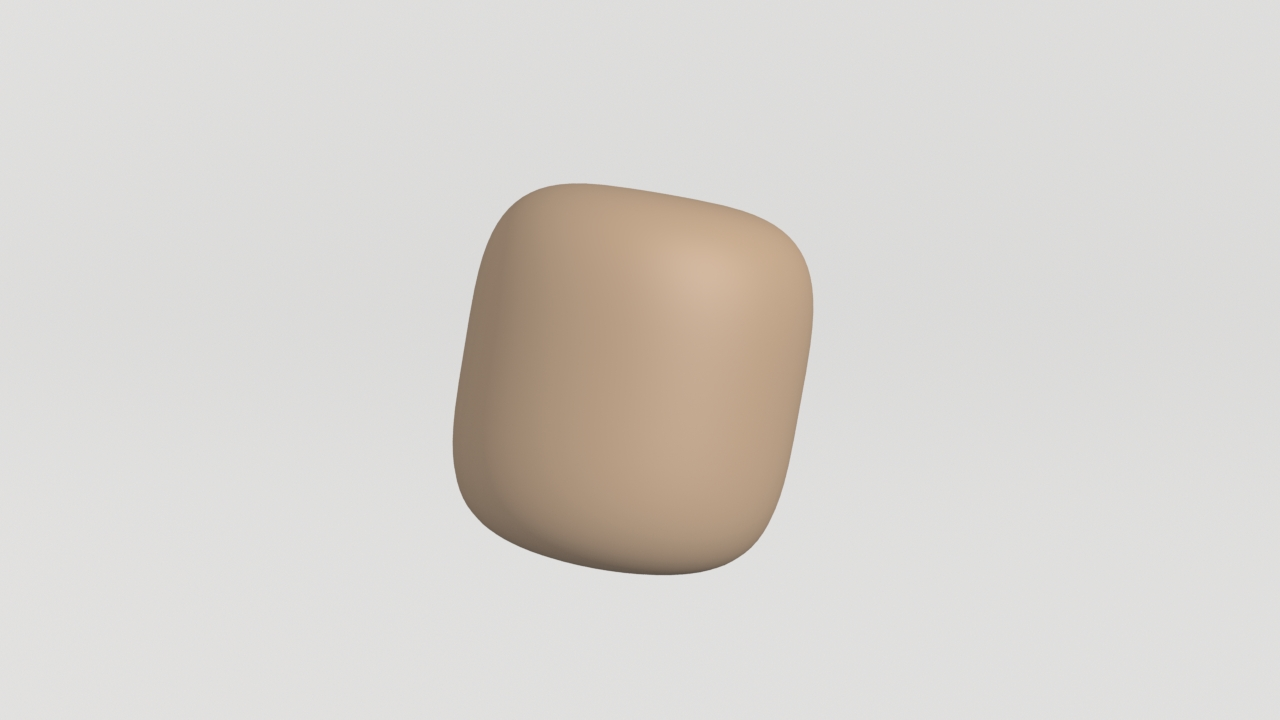
\includegraphics[height=0.8in]{./figure/torso_primitive.jpg}\caption{}\label{fig:torso_cylinder}
   \end{subfigure}
   \begin{subfigure}[t]{0.45\linewidth}
   \centering
       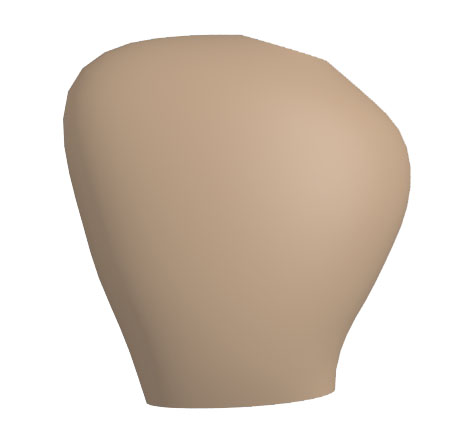
\includegraphics[height=0.8in]{./figure/torso_after_deformed.jpg}\caption{}\label{fig:torso_finish}
   \end{subfigure}
\caption{Primitive deformer: a) female warrior torso represented with a cylinder and its 2D silhouette contour, b) deformed shape of the cylinder }
 \label{fig:torso}
\end{figure}\\
Figure \ref{fig:torso}\subref{fig:torso_cylinder} depicts an arm model of the female warrior which is represented with a cylinder. The 2D silhouette contour to be matched is also shown in the image. Figure \ref{fig:torso}\subref{fig:torso_finish} shows how the cylinder is deformed with the algorithm developed below to match the 2D silhouette contour exactly. This is achieved by a sketch-guided and ODE-drive primitive deformer. It is developed from a simplified version of the Euler-Lagrange PDE (partial differential equation) which is widely used in physically-based surface deformations and briefly introduced below.\\
As discussed in \cite{botsch2008linear}, the main requirement for physically-based surface deformations is an elastic energy which considers locally stretching for solid objects plus bending for two-manifold surfaces called thin-shells. When a surface $\mathbb{S} \subset \mathbb{R}^3$ parameterized by a function $\mathbf{P(u,v)}: \Omega \subset  \mathbb{R}^2 \mapsto \mathbb{S} \subset \mathbb{R}^3 $is deformed to a new shape $\mathbb{S'}$ through adding a displacement vector $\mathbf{d(u,v)}$ to each point $\mathbf{P(u,v)}$, the change of the first and second fundamental $I(u,v),\Pi(u,v) \in \mathbb{R}^{2\times2}$,forms in differential geometry \cite{do2017differential} yields a measure of stretching and bending descried by \cite{terzopoulos1987elastically}\\
\begin{equation}
E_{shell}(S') = \int_{\Omega}k_s\|I'-I\|_F^2 +k_b\|\Pi'-\Pi\|_F^2 dudv \label{energy}
\end{equation}
Where ,$I'$,$\Pi'$ are the first and second fundamental forms of the surface $\mathbf{S'}$,  $ \| . \|$ indicates a (weighted) Frobenius norm, and the stiffness parameters $k_s$  and $k_b$ are used to control the resistance to stretching and bending. \\
Generating a new deformed surface requires the minimization of the above equation which is non-linear and computationally too expensive for interactive applications. In order to avoid the nonlinear minimization, the change of the first and second fundamental forms is replaced by the first and second order partial derivatives of the displacement function $\mathbf{d(u,v)}$ (Celniker, 1991), (Welch, 1992) , i. e.,   \\
\begin{equation}
\begin{aligned}
\tilde{E}_{shell}(d)&= \int_{\Omega}k_s(\|d_u\|^2+\|d_v\|^2) \\
&+k_b(\|d_{uu}\|^2+2\|d_{uv}\|+\|d_{vv}\|^2) dudv \label{energydiffgeo}
\end{aligned}
\end{equation}
where $d_x=\frac{\partial}{\partial{x}}$ and $d_{xy}=\frac{\partial^2}{\partial{x}\partial{y}}$ .
The minimization of the above equation can be obtained by applying variational calculus which leads to the following Euler-Lagrange PDE\\
\begin{equation}
-k_s\triangle d+k_b\triangle^2d=0
\label{lagrange}
\end{equation}
where $\triangle$ and $\triangle^2$ are the Laplacian and the bi-Laplacian operator, respectively.
\begin{equation}
\begin{aligned}
&\triangle d=div\nabla d=d_{uu}+d_{vv} \\
&\triangle^2d=\triangle(\triangle d) =d_{uuuu}+2d_{uuvv}+d_{vvvv}
\label{laplacianoperator}
\end{aligned}
\end{equation}\\
Using the sketched 2D silhouette contours shown in Figure \ref{fig:leg}\subref{fig:leg_cylinder} to change the shape of the primitive can be transformed into generation of a sweeping surface which passes through the two sketched 2D silhouette contours. The generator creating the sweeping surface is a curve of the parametric variable $u$ only, and the two silhouette contours are trajectories. If Equation \eqref{lagrange} is used to describe the generator, the parametric variable  in Equation \eqref{lagrange} drops, and we have  $d_{vv}=0$ and $d_{vvvv}=0$. Substituting  and  into Equation \eqref{lagrange}, we obtain the following simplified version of the Euler-Lagrange PDE \eqref{lagrange}which is actually a vector-valued ordinary differential equation
\begin{equation}
k_b\frac{\partial^4d}{\partial u^4}-k_s\frac{\partial^2 d}{\partial u^2}=0
\label{ODE}
\end{equation}\\
As pointed out in \cite{chaudhry2013shape} and \cite{chaudhry2015dynamic} , the finite difference solution of ordinary differential equations is very efficient, we here investigate such a numerical solution of Equation \eqref{laplacianoperator}. \\
\begin{figure}[h]
	\begin{center}
	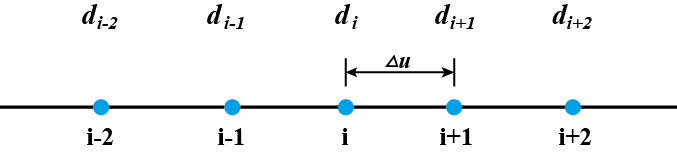
\includegraphics[width=0.8\columnwidth]{./figure/FDM.png}
	\caption{Typical node i  for the finite difference approximations of derivatives}
	\label{fig:fdm}
	\end{center}
\end{figure}\\
For a typical node  shown in Figure \ref{fig:fdm}, the central finite difference approximations of the second and fourth order derivatives can be written as \cite{chaudhry2013shape}
\begin{equation}
\begin{split}
\frac{\partial^2d}{\partial u^2}|_i &=\frac{1}{\triangle u^2}(d_{i+1}-2d_i+d_{i+1}) \\
\frac{\partial^4d}{\partial u^4}|_i &=\frac{1}{\triangle u^4}[6d_i-4(d_{i-1}+d_{i+1})+d_{i-2}+d_{i+2}]
\label{FDM}
\end{split}
\end{equation}\\
Introducing Equation \eqref{FDM} into Equation \eqref{ODE}, the following finite difference equation at the representative node $i$ can be written as:
\begin{equation}
\begin{split}
(6k_b+2k_sh^2)d_i+k_bd_{i-2}+k_bd_{i+2} \\
-(4k_b+k_sh^2)d_{i-1}-(4k_b+k_sh^2)d_{i+1}=0
\end{split}
\label{odefdm}
\end{equation}\\
For character models, the 3D shape defined by two silhouette contours is closed in the parametric direction u as indicated in Figure \ref{fig:FDMnode}\subref{fig:fdmnode_top}. Therefore, we can extract some closed curves each of which passes through the two corresponding points on the two silhouette contours. Taking the silhouette contours in Figure \ref{fig:FDMnode}\subref{fig:fdmnode_top} as an example, we find two corresponding points $\mathbf{c_{13}}$ and $\mathbf{c_{23}}$ on the original silhouette contours $\mathbf{c_1}$ and $\mathbf{c_2}$, and two corresponding points $\mathbf{c'_{13}}$ and $\mathbf{c'_{23}}$ on the deformed silhouette contours $\mathbf{c'_1}$ and $\mathbf{c'_2}$ as shown in Figure \ref{fig:FDMnode}\subref{fig:fdmnode_top}. Then we extract a closed curve $\mathbf{c(u)}$ passing through the two corresponding points $\mathbf{c_{13}}$ and $\mathbf{c_{23}}$ from the 3D model in Figure \ref{fig:FDMnode}\subref{fig:fdmnode_side} and depicted it as a dashed curve in Figure \ref{fig:FDMnode}(b). Assuming that the deformed shape of the closed curve $\mathbf{c(u)}$ is $\mathbf{c'(u)}$, the displacement difference between the original closed curve and deformed closed curve is $\mathbf{d(u)=c'(u)-c(u)}$. Our task is to find the displacement difference $\mathbf{d(u)}$ and generate the deformed curve $\mathbf{c'(u)=d(u)+c(u)}$.
\begin{figure}[h]
\begin{center}
  \begin{subfigure}[!b]{0.45\linewidth}
       \centering
       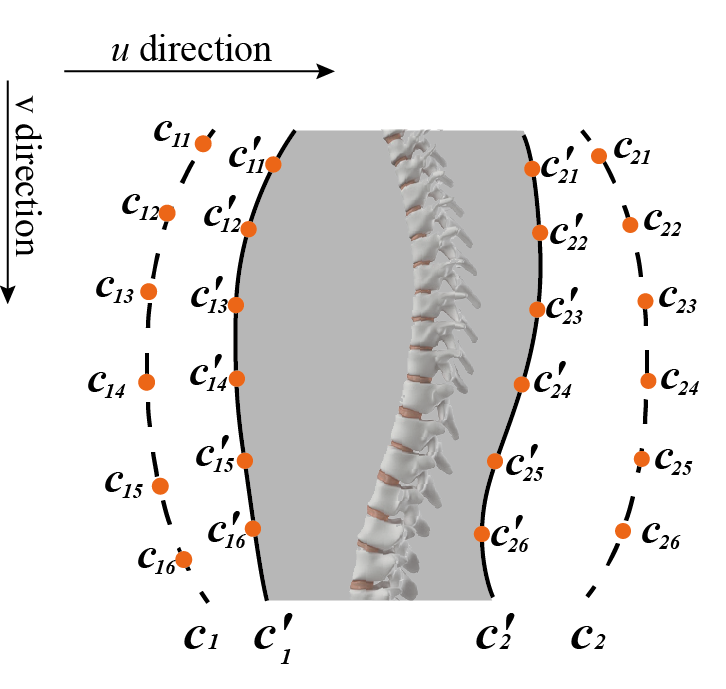
\includegraphics[width=0.9\linewidth]{./figure/fdmnode_a.png}
        \caption{side view}\label{fig:fdmnode_side}
   \end{subfigure}
   \begin{subfigure}[!b]{0.45\linewidth}
       \centering
       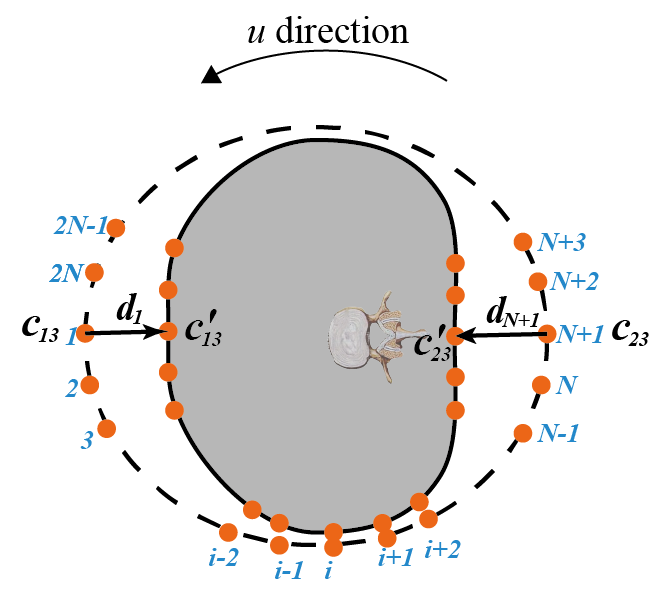
\includegraphics[width=0.9\linewidth]{./figure/fdmnode_b.png}
        \caption{top view}\label{fig:fdmnode_top}
   \end{subfigure}
%      \begin{subfigure}[!b]{0.9\linewidth}
%       \centering
%       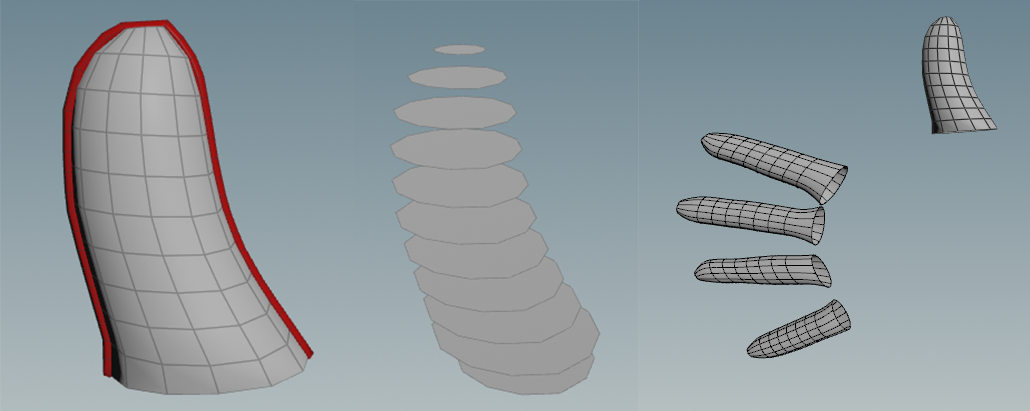
\includegraphics[width=0.9\linewidth]{./figure/finger_group.png}
%        \caption{the making of the fingers}\label{fig:fingers}
%   \end{subfigure}
	\caption{Finite difference nodes for local shape manipulation from sketches in different view planes and the deformed 3D finger models}
	\label{fig:FDMnode}
	\end{center}
\end{figure}\\
In order to use the finite difference method to find the displacement difference $\mathbf{d(u)}$, we uniformly divide the closed curve into $2N$ equal interval as indicated in Figure \ref{fig:FDMnode}. The displacement difference at node 1 and node $\mathbf{N}$ is known, i. e. $\mathbf{d_1=c'_{13}-c_{13}}$ and $\mathbf{d_{N+1}=c'_{23}-c_{23}}$. \\
When we write the finite difference equations for the nodes 2, 3, $2N-1$ and $2N$, the node 1 will be involved, and we have  $\mathbf{d_1=c'_{13}-c_{13}}$. The finite difference equations at these points can be derived from Equation \eqref{odefdm}. Substituting  $\mathbf{d_1=c'_{13}-c_{13}}$ into these equations, we obtain the finite difference equations for the nodes 2, 3, $2N-1$ and $2N$\\%, and present them in Appendix A. 
When we write the finite difference equations for the nodes $N-1$,$N$, $N+2$ and $N+3$, the node $N+1$ will be involved, and we have $\mathbf{d_{N+1}=c'_{23}-c_{23}}$. Once again, the finite difference equations at these points can be derived from Equation \eqref{odefdm}. Substituting $\mathbf{d_{N+1}=c'_{23}-c_{23}}$ into these equations, we obtain the finite difference equations for the nodes N-1, N, N+2 and N+3\\%, and present them in Appendix A as well. 
For all other nodes 3, 4, 5,\ldots, $N-3$ , $N-2$ and $N+4$,$N+5$ ,\ldots, $2N-3$, $2N-2$, the finite difference equations are the same as Equation \eqref{odefdm}. For these nodes, there are $2N-5$ finite difference equations. Plus the 8 finite difference equations at node 2, 3, $N-1$ , $N$ , $N+2$ , $N+3$ , $2N-1$ and $2N$, we get  $2N-2$linear algebra equations which can be solved to determine the  unknown constants $\mathbf{d_2}$, $\mathbf{d_3}$ , \ldots,$\mathbf{d_{N-1}}$, $\mathbf{d_{N}}$ , $\mathbf{d_{N+2}}$ , $\mathbf{d_{N+3}}$ ,\ldots, $\mathbf{d_{2N-1}}$, and $\mathbf{d_{2N}}$. Adding the $\mathbf{d_i}$ ( $i=1,2,\ldots,2N-1,2N$) to the original curve $\mathbf{c(u)}$, we obtain the deformed curve $\mathbf{c'(u)}$, and depict it as a solid curve in Figure \ref{fig:FDMnode}\subref{fig:fdmnode_top}. Repeating the above operations for all other points on the two silhouette contours, we obtain all deformed curves. These curves describe a new 3D deformed shape.\\
%Taking a finger shown in Figure \ref{fig:FDMnode}\subref{fig:fingers} as an example, the left image shows the silhouette contours. It is used deform a cylinder into the middle 3D model (the second image from the left). The cross-section shapes of the finger model are depicted in the third image from the left. The rightmost image shows the five finger models created with the above method.\\
With the primitive deformer developed above, we deform the primitive of the 3D base mesh shown in Figure \ref{fig:system_overview}\subref{fig:superellipsoid_primitives}, obtain a deformed 3D base mesh, and depicted it in Figure \ref{fig:system_overview}\subref{fig:primitives_after_deformation}. It is clear that deformed primitives have matched the generated 2D silhouette contours exactly. \\% We have also deformed the primitives to match the silhouette contours of the Knight sketches shown in Figure 6(a), and obtain the deformed 3D base mesh of the knight model shown in Figure 6(b). 
\section{Detail generator}\label{detail_generator}
In order to add 3D details to 3D base mesh created from the primitive generator, we develop a detail generator consisting of a local shape creator and an image-based detail generator. In what follows, we first introduce the user interface of our developed detail generator in Subsection\ref{user_interface_of_detail_generator}. Then we discuss the local shape creator in Subsection\ref{local_shape_creator}.
\subsection{User interface of detail generator}\label{user_interface_of_detail_generator}
The user interface of our developed detail generator uses different windows. They are used to respectively treat local model creation from sketches in different view planes, and 2D image-based detail generation.
For local model creation, four windows are used to help provide depth information and control the shape of 3D local details to be created. As shown in Figure 7, the two top windows and left bottom window allow users to sketch 2D silhouette contours from two or all of three orthotropic views: front view, side view, and top view in the local coordinates of a local shape, or project a 3D model to the three orthotropic views to modify them. The right bottom window is used to display the created 3D models.\\
\begin{figure}[h]
\centering
       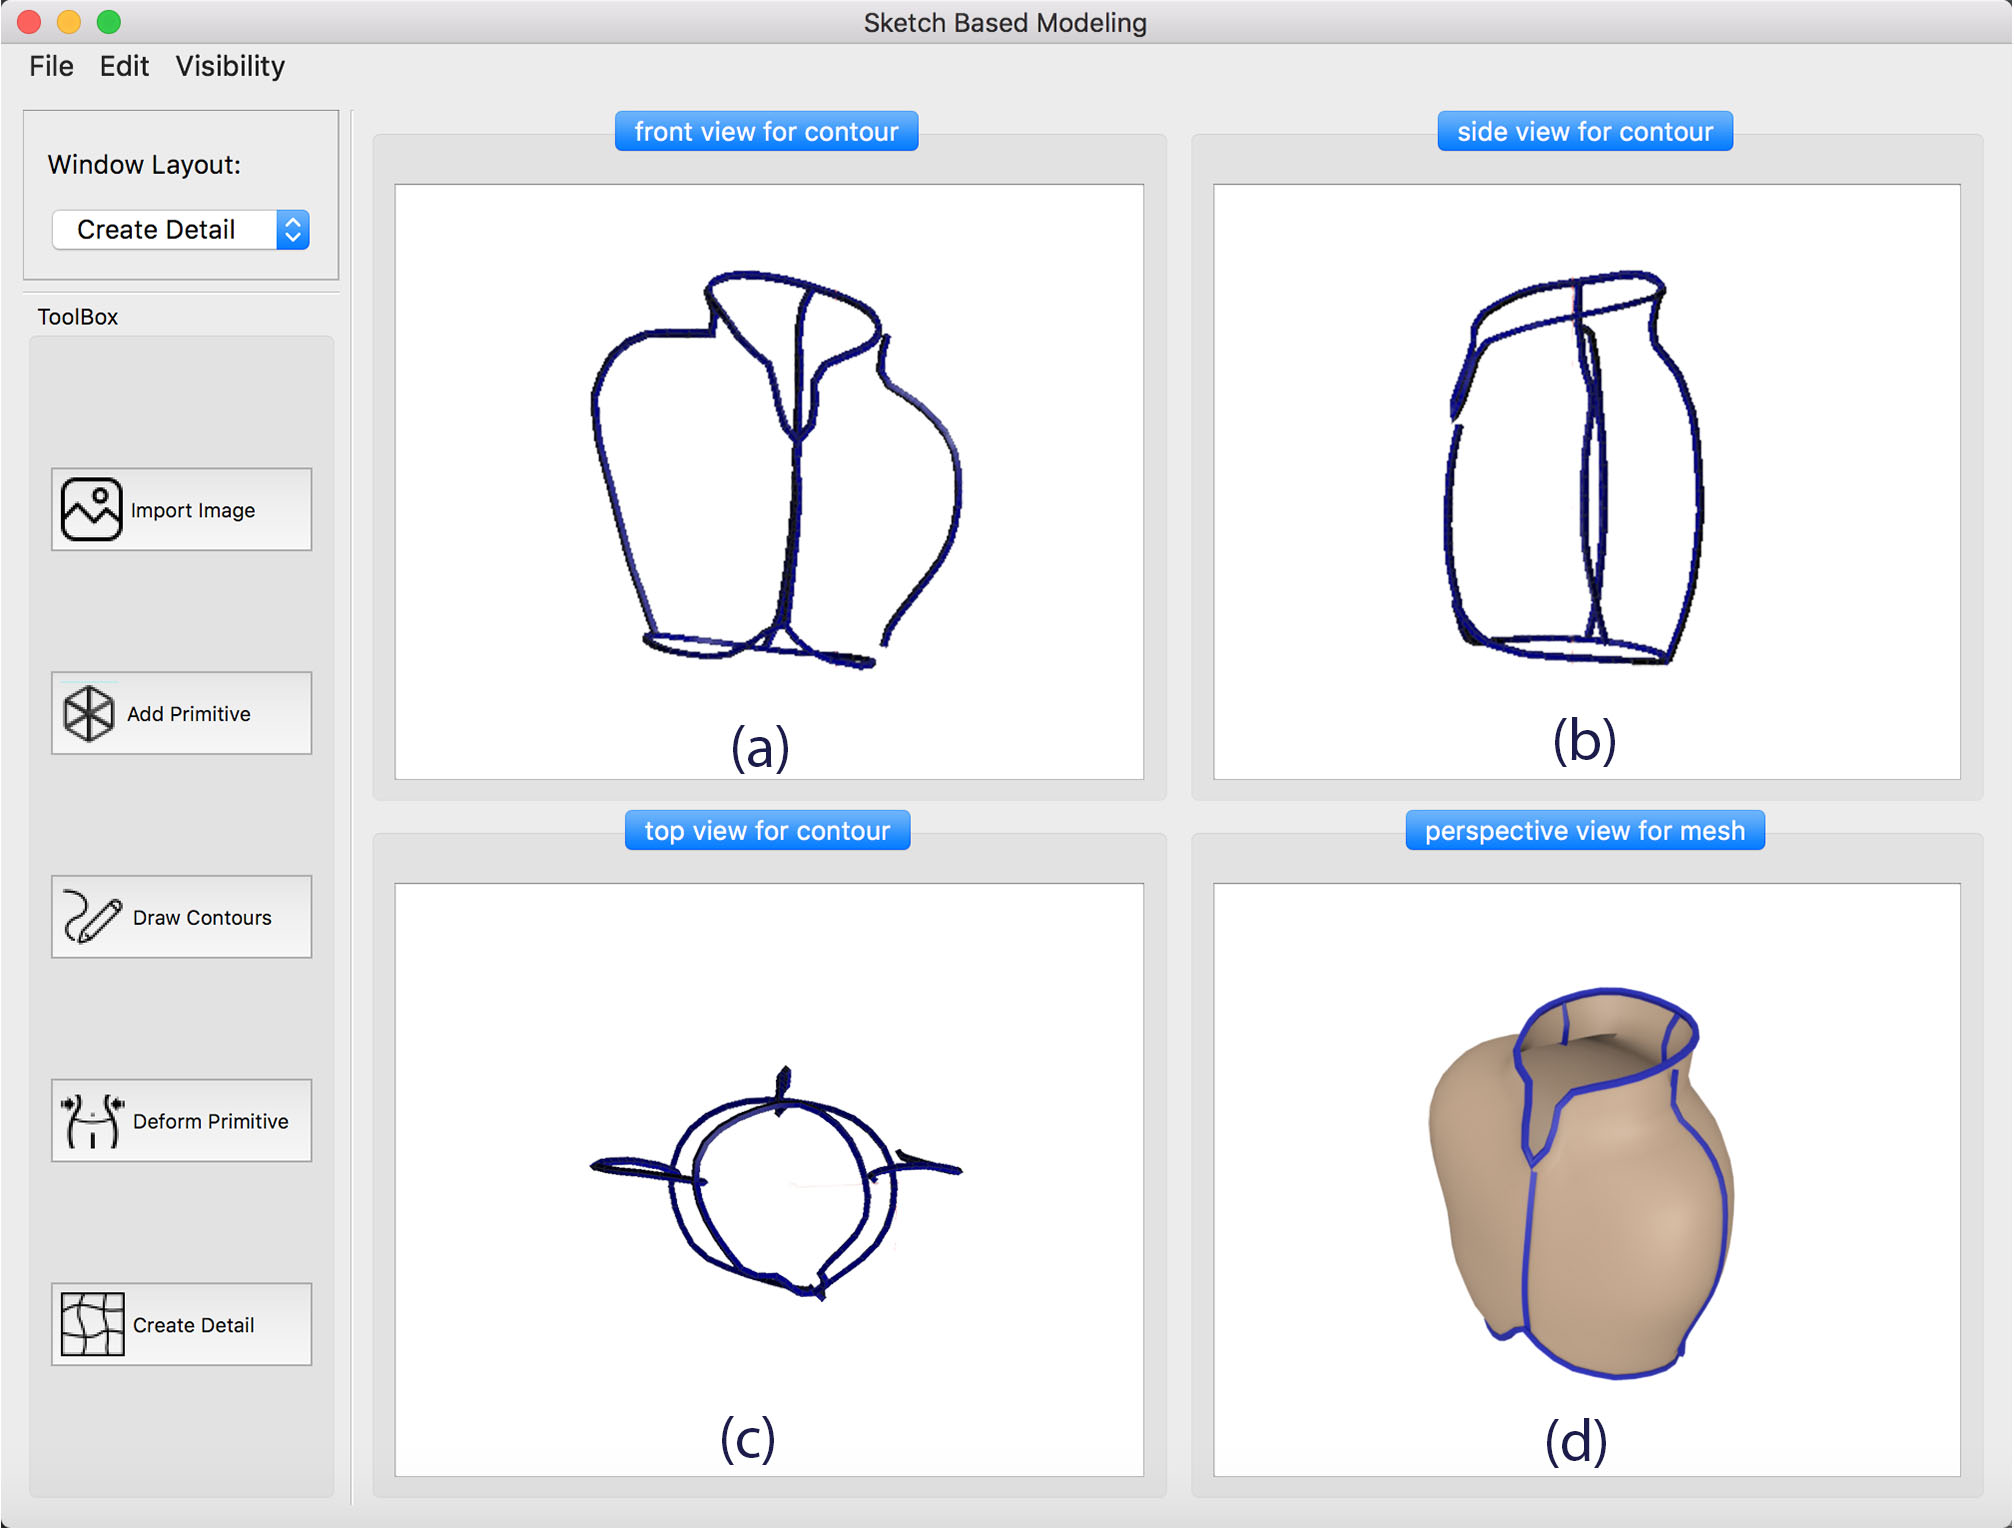
\includegraphics[width=1.0\linewidth]{./figure/detail_UI.jpg}
\caption{Interface for sketching three orthotropic silhouette contours and viewing generated 3D models}
 \label{fig:detail_UI}
\end{figure}
%Taking the upper body model as an example, we first sketch a 2D silhouette contour in the front view window as indicted in the upper left part in Figure \ref{fig:detail_UI}. The sketched silhouette contour is also displayed in the side view window, which locates at the upper right part of the Figure \ref{fig:detail_UI}. Then we sketch the second 2D silhouette contour in the side view window which intersects with the 2D silhouette contour in the front view window. Both the 2D silhouette contours sketched in the front and side view windows are displayed in the top view window in the lower left part of Figure \ref{fig:detail_UI}. In the top view window, we sketch the third 2D silhouette contour shown which intersects with the two sketched silhouette contours respectively obtained from the front view and the side view. Once a 3D model is created from the two or three sketched silhouette contours, it is displayed in the right bottom window. \\
Taking the breast model as an example, we first sketch a 2D silhouette contour in the front view window as indicted in the upper left part in Figure \ref{fig:detail_UI}. The sketched silhouette contour is also displayed in the side view window and top view window, which locate at the upper right part of the Figure \ref{fig:detail_UI} and lower left part of the Figure \ref{fig:detail_UI}, respectively. Then one can manipulate the 2D silhouette contours in all three views to your heart's content. Once a 3D model is created from the two or three sketched silhouette contours, it is displayed in the right bottom window of Figure \ref{fig:detail_UI}. \\
For 2D image-based detail generation, 2D images are input into the left window. After carrying out the calculations of shape-from-shading, the generated 3D models are displayed in the right windows. Users can input a whole character model into the window and perform the operations of adding the generated models to the whole character model.
\subsection{local shape creator}\label{local_shape_creator}
Although a 3D regional model can be created from two sketched silhouette contours in the same view plane as discussed in Subsection \ref{algorithm_of_primitive_deformer}, the shape changes in the depth direction may not be our expected ones. In order to allow users to control shape changes in the depth direction and smoothly connect primitives together, we develop a new local shape creator to create a 3D model from two or three silhouette contours in different view planes. It is developed from the four algorithms which can create a model from two open sketches, one open and one closed sketches, two open and one closed sketches, and two closed curves, respectively. In the following four subsections, we will investigate these four algorithms. 
\subsubsection{Algorithm for two open silhouette contours in two different view planes}\label{algorithm_2_opens}
For creation of a local 3D model from two open silhouette contours in two different view planes, we use the intersecting point  $\mathbf{p}$ to segment each of the two sketched 2D silhouette contours obtained from the front view and the side view into two curves and denote all the four segmented curves with  $\mathbf{c_1}$, $\mathbf{c_2}$ , $\mathbf{c_3}$ and $\mathbf{c_4}$. Then we find the four corresponding points from the four curves, and denote them with $\mathbf{c_{1j}}$, $\mathbf{c_{2j}}$, $\mathbf{c_{3j}}$ and $\mathbf{c_{4j}}$, respectively as shown in Figure \ref{fig:2open}. Since the four points are on the two sketched 2D silhouette contours in the front view and the side view, their coordinate values are known. \\
\begin{figure}[h]
	\begin{center}
  \begin{subfigure}[b]{0.45\linewidth}
       \centering
       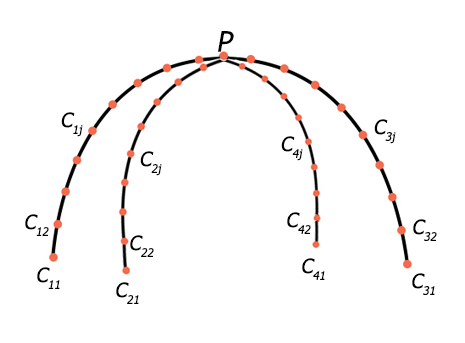
\includegraphics[width=\linewidth]{./figure/2opens_a.jpg}
        \caption{side view}\label{fig:2opens_side}
   \end{subfigure}
   \begin{subfigure}[b]{0.45\linewidth}
       \centering
       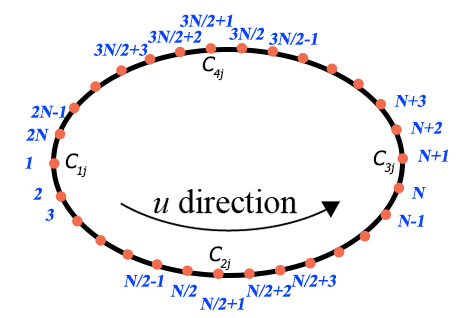
\includegraphics[width=0.9\linewidth]{./figure/2opens_b.jpg}
        \caption{top view}\label{fig:2opens_top}
   \end{subfigure}
	\caption{Finite difference nodes for the algorithm for two open silhouette contours in two different view planes}
	\label{fig:2open}
		\end{center}
\end{figure}\\
The 3D model to be created from the two sketched 2D silhouette contours can be regarded as a sweeping surface whose generator is a closed curve $\mathbf{c(u)}$ shown in Figure \ref{fig:2open}\subref{fig:2opens_top} passing through the four corresponding points $\mathbf{c_{1j}}$ , $\mathbf{c_{2j}}$ , $\mathbf{c_{3j}}$ and $\mathbf{c_{4j}}$,  and shown in Figure \ref{fig:2open}(a) and (b). We uniformly divide the domain of the parametric variable $u$ corresponding to the closed curve (generator) $\mathbf{c(u)}$ into $2N$ equal intervals. The nodes corresponding to $\mathbf{c_{1j}}$ , $\mathbf{c_{2j}}$ , $\mathbf{c_{3j}}$ and $\mathbf{c_{4j}}$ are 1, $N/2+1$ , $N+1$ and $3/2N+1$ , respectively as demonstrated in Figure \ref{fig:2open}(b). Here, the selection of  $N$ should ensure that  is an even number and $N\geqslant4$. \\
The finite difference equations for the nodes 4, 5, \ldots, $N/2-3$, $N/2-2$; $N/2+4$, $N/2+5$, \ldots, $N-3$, $N-2$; $N+4$, $N+5$, \ldots, $3N/2-3$, $3N/2-2$; $3N/2+2$, $3N/2+3$, \ldots, $2N-3$, and $2N-2$ are the same as Equation \eqref{odefdm}.\\
The finite difference equations for the nodes 2, 3, $N/2-1$, $N/2$, $N/2+2$, $N/2+3$, $N-1$, $N$, $N+2$, $N+3$, $3N/2-1$, $3N/2$, $3N/2+2$, $3N/2+3$, $2N-1$, and $2N$ can be obtained by introducing the corresponding one of $\mathbf{c_{1j}}$, $\mathbf{c_{2j}}$ , $\mathbf{c_{3j}}$ and $\mathbf{c_{4j}}$ into Equation \eqref{odefdm} to replace $d_1$ , $d_{N/2+1}$ , $d_{N+1}$ and $d_{3N/2+1}$ accordingly. \\%The finite difference equations for these nodes are given in Appendix B.
Putting all obtained finite difference equations together, we obtain all the unknown constants $\mathbf{d_2}$ , $\mathbf{d_3}$ , \ldots, $\mathbf{d_{N/2-1}}$ , $\mathbf{d_{N/2}}$ , $\mathbf{d_{N/2+2}}$, $\mathbf{d_{N/2+3}}$ , \ldots , $\mathbf{d_{N-1}}$ , $\mathbf{d_N}$ , $\mathbf{d_{N+2}}$ , $\mathbf{d_{N+3}}$ ,\ldots, $\mathbf{d_{3N/2-1}}$ , $\mathbf{d_{3N/2}}$ , $\mathbf{d_{3N/2+2}}$ , $\mathbf{d_{3N/2+3}}$ , \ldots , $\mathbf{d_{2N-1}}$ and $d_{2N}$ . They together with the known four points $\mathbf{c_{1j}}$, $\mathbf{c_{2j}}$ , $\mathbf{c_{3j}}$ and $\mathbf{c_{4j}}$ are used to define the generator.\\
Repeating the above treatment for all other points on the four curves $\mathbf{c_1}$ , $\mathbf{c_2}$ , $\mathbf{c_3}$ and $\mathbf{c_4}$, we obtain the generators at the other positions. With these generators, we create local 3D shapes.
\begin{figure}[!hbt]
\centering
\begin{subfigure}{0.24\linewidth}
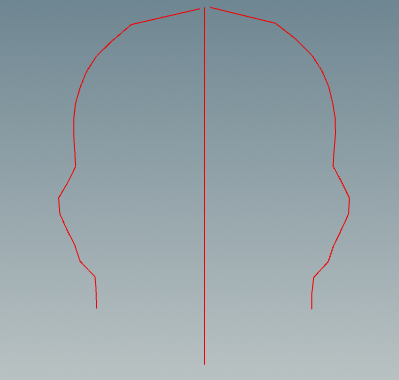
\includegraphics[height=0.9in]{./figure/headcontourfront.png}\caption{}\label{fig:head_contour_front}
\end{subfigure}
\begin{subfigure}{0.24\linewidth}
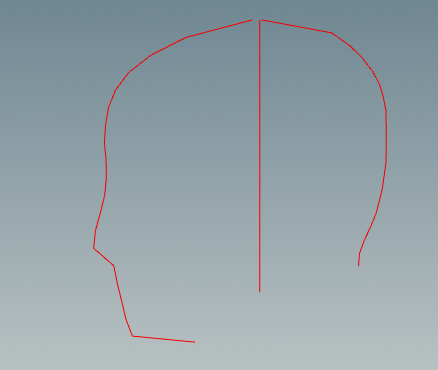
\includegraphics[height=0.9in]{./figure/headcontourside.png}\caption{}\label{fig:head_contour_side}
\end{subfigure}
\begin{subfigure}{0.24\linewidth}
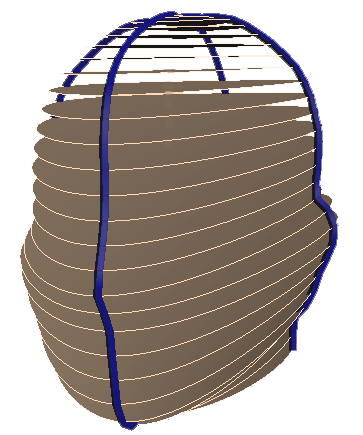
\includegraphics[height=0.9in]{./figure/head_cross_section.png}\caption{}\label{fig:head_cross_section}
\end{subfigure}
\begin{subfigure}{0.24\linewidth}
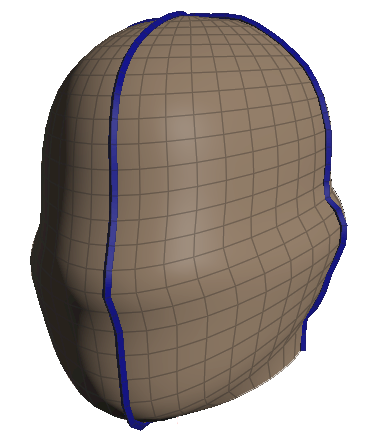
\includegraphics[height=0.9in]{./figure/head_final.png}\caption{}\label{fig:head_mesh}
\end{subfigure}
\caption{Primitive generator: a) 2D silhouette contours of the male head in front view, b)-2D silhouette contours of the male head in front view, c) cross sections of the male head d) lofting the cross sections into a male head mesh}
\label{fig:head}
\end{figure}\\
A head model is used to demonstrate the above method Figure \ref{fig:head}. Figure \ref{fig:head}\subref{fig:head_contour_front} and Figure \ref{fig:head}\subref{fig:head_contour_side} show two open head silhouette contours in two different view plans. Figure \ref{fig:head}\subref{fig:head_cross_section} shows the cross section for each discrete parameter $u_i$. Figure \ref{fig:head}\subref{fig:head_mesh} depicted the created 3D head model. \\
The above method can be directly extended to deal with local shape creation from four disconnected silhouette contours. The silhouette contours of the leg model in the front and side views are shown in Figure \ref{fig:male_leg}\subref{fig:leg_contour_front} and Figure \ref{fig:male_leg}\subref{fig:leg_contour_side}, respectively. The corresponding four points on the four silhouette contours are used to define a cross-section curve. All of these cross section curves are used to generate the 3D leg model with the front and side views in Figure \ref{fig:male_leg}\subref{fig:leg_mesh_front} and Figure \ref{fig:male_leg}\subref{fig:leg_mesh_side}, respectively.  Another example given in Figure \ref{fig:male_leg} is a neck generated in the same fashion where Figure \ref{fig:male_leg}\subref{fig:neck_contour} shows the 4 disconnected contours, Figure \ref{fig:male_leg}\subref{fig:neck_cross_section} shows the cross-sections for each discrete $u$ and finally the mesh is in Figure \ref{fig:male_leg}\subref{fig:neck_mesh}
\begin{figure}[h!tb]
\centering
\begin{subfigure}{0.24\linewidth}
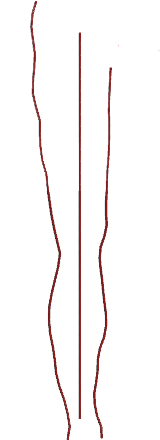
\includegraphics[height=1.9in]{./figure/legcontourfront.png}\caption{}\label{fig:leg_contour_front}
\end{subfigure}
\begin{subfigure}{0.24\linewidth}
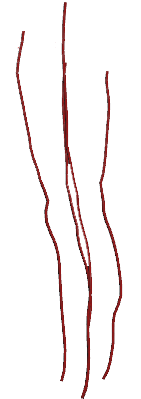
\includegraphics[height=1.9in]{./figure/legcontourside.png}\caption{}\label{fig:leg_contour_side}
\end{subfigure}
\begin{subfigure}{0.24\linewidth}
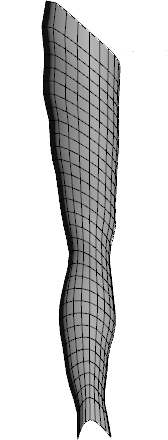
\includegraphics[height=1.9in]{./figure/legfront.png}\caption{}\label{fig:leg_mesh_front}
\end{subfigure}
\begin{subfigure}{0.24\linewidth}
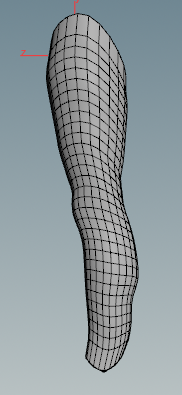
\includegraphics[height=1.9in]{./figure/legside.png}\caption{}\label{fig:leg_mesh_side}
\end{subfigure}
\begin{subfigure}{0.32\linewidth}
\centering
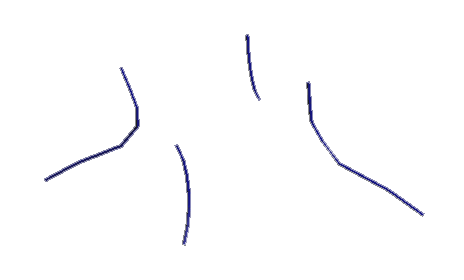
\includegraphics[height=0.7in]{./figure/neck_contour.png}\caption{}\label{fig:neck_contour}
\end{subfigure}
\begin{subfigure}{0.32\linewidth}
\centering
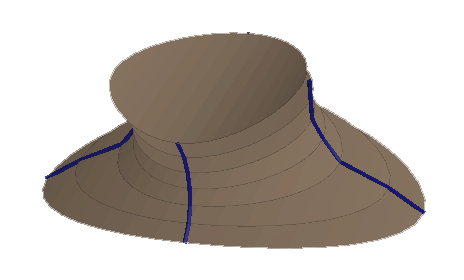
\includegraphics[height=0.7in]{./figure/neck_cross_section.png}\caption{}\label{fig:neck_cross_section}
\end{subfigure}
\begin{subfigure}{0.32\linewidth}
\centering
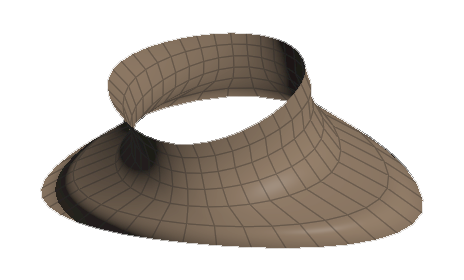
\includegraphics[height=0.7in]{./figure/neck_mesh.png}\caption{}\label{fig:neck_mesh}
\end{subfigure}
\caption{leg model creation from two open silhouette contours in two different view planes}
\label{fig:male_leg}
\end{figure}\\
%\begin{figure}[!htb]
%\begin{center}
%\begin{subfigure}{0.32\linewidth}
%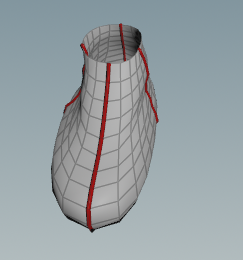
\includegraphics[height=1in]{./figure/foot2.png}\caption{}\label{fig:foot_mesh}
%\end{subfigure}
%\begin{subfigure}{0.32\linewidth}
%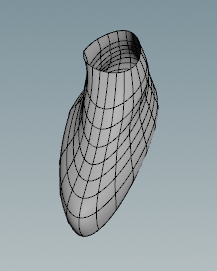
\includegraphics[height=1in]{./figure/foot1.png}\caption{}\label{fig:foot_failed_mesh}
%\end{subfigure}
%\begin{subfigure}{0.32\linewidth}
%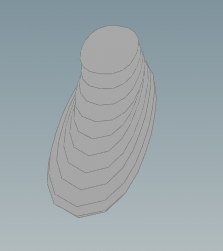
\includegraphics[height=1in]{./figure/foot_scale_cross-section.png}\caption{}\label{fig:foot_cross_section}
%\end{subfigure}
%\hfill
%\begin{subfigure}{0.65\linewidth}
%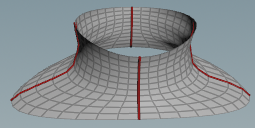
\includegraphics[height=1in]{./figure/neck.png}\caption{}\label{fig:neck}
%\end{subfigure}
%\begin{subfigure}{0.3\linewidth}
%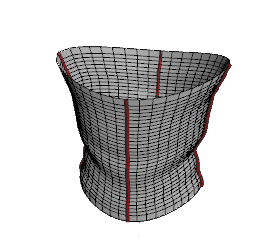
\includegraphics[height=1in]{./figure/torso.png}\caption{}\label{fig:lower_torso}
%\end{subfigure}
%\caption{Creation of 3D foot, neck, and torso models from two open silhouette contours in two different view planes}
%\label{fig:more_example_on_2opens}
%\end{center}
%\end{figure}
%More modeling examples are given in Figures \ref{fig:more_example_on_2opens}. Figure \ref{fig:more_example_on_2opens}\subref{fig:foot_mesh} shows the four silhouette contours of a foot model in the front and side views. Figure \ref{fig:more_example_on_2opens}\subref{fig:foot_failed_mesh} depicts the 3D foot model created from the four silhouette contours. Figure \ref{fig:more_example_on_2opens}\subref{fig:foot_cross_section} shows the cross-section curves. Figures \ref{fig:more_example_on_2opens}\subref{fig:neck} and \ref{fig:more_example_on_2opens}\subref{fig:lower_torso} give 3D neck model and torso model generated from the above method.\\
\subsubsection{Algorithm for one open and one closed silhouette contours in two different view planes}\label{algorithm_1_open_1_closed}
For creation of a local 3D model from one open and one closed silhouette contours in two different view plans as shown in Figure \ref{fig:1open1close}, the intersecting points $\mathbf{p_1}$ and $\mathbf{p_3}$ between the open silhouette contour and the closed silhouette contour divide the closed silhouette contour into two curves. Then we find the middle points $\mathbf{p_2}$ and $\mathbf{p_4}$ of the two curves. These four points $\mathbf{p_1}$ , $\mathbf{p_2}$ , $\mathbf{p_3}$ and $\mathbf{p_4}$ divide the closed silhouette contour into four curves $\mathbf{c_1}$ , $\mathbf{c_3}$ , $\mathbf{c_4}$ and $\mathbf{c_6}$ . Next, we find the middle point $\mathbf{p}$ of the open silhouette contour which divides the open silhouette contour into two curves $\mathbf{c_2}$ and $\mathbf{c_5}$. With this treatment, the creation of the local 3D detail model is changed into creation of two sweeping surfaces: one is defined by the three curves $\mathbf{c_1}$ , $\mathbf{c_2}$ and $\mathbf{c_3}$ , and the other is defined by the three curves $\mathbf{c_4}$ , $\mathbf{c_5}$ and $\mathbf{c_6}$ . \\
Since the creation process of the two weeping surfaces is the same, we take the creation of the sweeping surface defined by the three curves $\mathbf{c_1}$ , $\mathbf{c_2}$ and $\mathbf{c_3}$ to demonstrate the process.\\
For each of the three curves $\mathbf{c_1}$ , $\mathbf{c_2}$ and $\mathbf{c_3}$ we uniformly divide it into $2N$ equal intervals, and use $\mathbf{c_{1j}}$, $\mathbf{c_{2j}}$ and $\mathbf{c_{3j} (j=1,2,\ldots,J)}$ to respectively indicate the nodes on the three curves.\\
The sweeping surface can be generated by sweeping a generator $\mathbf{c(u)}$ passing through the points$\mathbf{c_{1j}}$, $\mathbf{c_{2j}}$ and $\mathbf{c_{3j}}$ . Based on this consideration, the creation of the sweeping surface is transformed into determination of the generator at different positions along the curve.\\
In order to create the generator $\mathbf{c(u)}$ passing the points $\mathbf{c_{1j}}$, $\mathbf{c_{2j}}$ and $\mathbf{c_{3j}}$, we uniformly divide the domain of the parametric variable $u$ corresponding to the generator $\mathbf{c(u)}$ into 2N equal intervals, and get the nodes 1, 2, \ldots, $2N-1$ , $2N$ and $2N+1$ . Since the nodes 1, $N+1$, and $2N+1$ are on the curves $\mathbf{c_1}$ , $\mathbf{c_2}$ and $\mathbf{c_3}$, their values are known, i. e.$\mathbf{d_1=c_{1j}}$ , $\mathbf{d_{N+1}=c_{2j}}$ and $\mathbf{d_{2N+1}=c_{3j}}$. When writing the finite difference equations for the node 2 and the node $2N$, the node 0 beyond the boundary node 1 and the node $2N+2$ beyond the boundary node $2N+1$ will be involved. They can be determined below.\\
If the created local 3D model is to be smoothly connected to another 3D model, we can obtain a closed curve close to but larger than the closed silhouette contour from another 3D model. Then, the vector-valued first derivative $\mathbf{T_{1j}}$ on the curve $\mathbf{c_1}$ and $\mathbf{T_{3j}}$ on the curve $\mathbf{c_3}$ can be calculated from the closed curve and the closed silhouette contour.\\
\begin{figure}[h!tb]
	\begin{center}
	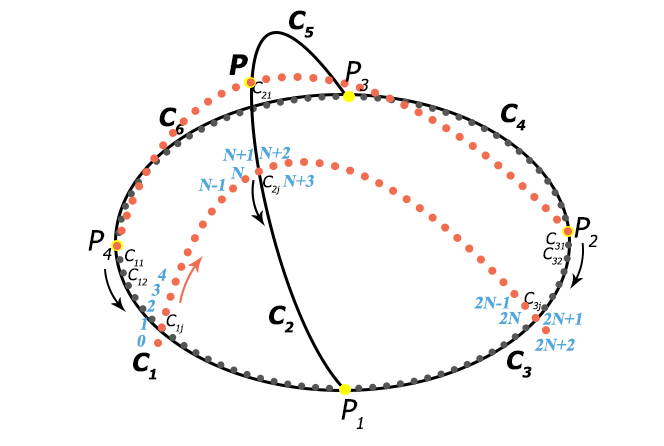
\includegraphics[width=0.7\columnwidth]{./figure/1open1close.jpeg}
	\end{center}
	\caption{Finite difference nodes for Algorithm for one open and one closed silhouette contours}
	\label{fig:1open1close}
\end{figure}
If the created local 3D model is to be connected to another 3D model with positional continuation only, the vector-valued first derivative $\mathbf{T_{1j}}$ on the curve $\mathbf{c_1}$ and $\mathbf{T_{3j}}$ on the curve $\mathbf{c_3}$ can be estimated from the three points $\mathbf{c_{1j}}$ , $\mathbf{c_{2j}}$ and $\mathbf{c_{3j}}$ by first constructing a curve passing through the three points and then calculating the vector-valued first derivative of the constructed curve at the points $\mathbf{c_{1j}}$ and $\mathbf{c_{3j}}$ . Once the vector-valued first derivatives $\mathbf{T_{1j}}$ and $\mathbf{T_{3j}}$ are obtained. The nodes 0 and $2N+2$ can be determined by the following finite difference approximation.\\
\begin{equation}
\mathbf{T_{1j}}=\frac{\mathbf{d_2-d_0}}{2\triangle u},      
\mathbf{T_{3j}}=\frac{\mathbf{d_{2N+2}-d_{2N}}}{2\triangle u} 
\label{tangent}
\end{equation}
Solving the above equation, we obtain the nodes 0 and $2N+2$ by
\begin{equation}
\begin{split}
\mathbf{d_0}=\mathbf{d_2}-2\mathbf{T_{1j}}\triangle u \\
\mathbf{d_{2N+2}}=\mathbf{d_{2N}}+2\mathbf{T_{3j}}\triangle u
\end{split}
\label{derivefromtangent}
\end{equation}
The finite difference equations for nodes 4, 5, \ldots, $N-3$, $N-2$ and $N+4$, $N+5$, \ldots, $2N-3$, $2N-2$ are the same as Equation \eqref{odefdm}. \\
The finite difference equations for the nodes 2, 3, $N-1$ , $N$ , $N+2$ , $N+3$ , $2N-1$ and $2N$ can be obtained by introducing the above equation and $\mathbf{d_1=c_{1j}}$ , $\mathbf{d_2=c_{2j}}$ and $\mathbf{d_3=c_{3j}}$ into Equation \eqref{odefdm}. \\%The obtained finite difference equations for these nodes are given in Appendix C.
Solving the finite difference equations for all the inner nodes 2, 3, \ldots , $2N-1$ and $2N$, we obtain all the unknown constants $d_2$ , $d_3$ , \ldots , $d_{2N-1}$ and $d_{2N}$. They together with the three known points $c_{1j}$ , $c_{2j}$ and $c_{3j}$ are used to create the generator.\\
Using the same treatment, we can obtain the generator at the other positions. From these obtained generators, a local detail 3D model is created and depicted in (b) of Figure \ref{fig:shoulder_armor}.\\
\begin{figure}[!htb]
\centering
\begin{subfigure}{0.24\linewidth}
\centering
\fbox{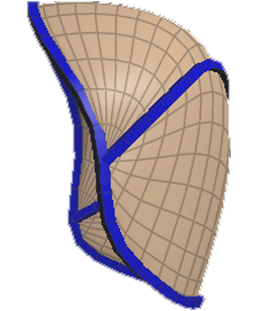
\includegraphics[height=0.7in]{./figure/shoulder_armor_front.png}}\caption{front}\label{shoulder_armor_front}
\end{subfigure}
\begin{subfigure}{0.24\linewidth}
\centering
\fbox{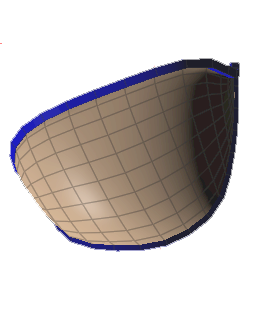
\includegraphics[height=0.7in]{./figure/shoulder_armor_top.png}}\caption{top}\label{shoulder_armor_top}
\end{subfigure}
\begin{subfigure}{0.24\linewidth}
\centering
\fbox{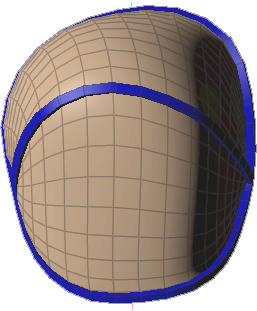
\includegraphics[height=0.7in]{./figure/shoulder_armor_side.png}}\caption{side}\label{shoulder_armor_side}
\end{subfigure}
\begin{subfigure}{0.24\linewidth}
\centering
\fbox{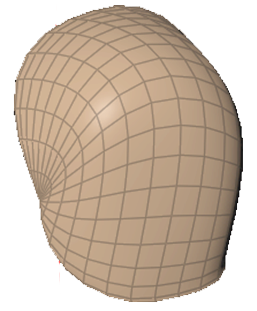
\includegraphics[height=0.7in]{./figure/shoulder_armor_persp.png}}\caption{perspective}\label{shoulder_armor_persp}
\end{subfigure}
\caption{creation of one open and one closed silhouette contours in four different view planes}
\label{fig:shoulder_armor}
\end{figure}
\subsubsection{Algorithm for two open and one closed silhouette contours in three different view planes}\label{algorithm_2_opens_1_close}
By introducing depth information, users can have more power to control the shape of the 3D model to be created as demonstrated by the algorithms given in Subsections \ref{algorithm_2_opens} and \ref{algorithm_1_open_1_closed}. Users can further control the shape of 3D models by using one or more silhouette contours in other view planes. In this subsection, we discuss construct a 3D detail model from two open and one closed silhouette contours in three orthotropic view planes.\\
As shown in Figure \ref{fig:2open1close}, the task of creating a local 3D detail model passing through two open and one closed silhouette contours can be transformed into constructing 4 sweeping surfaces encircled by the curves $\mathbf{c_1c_6c_5}$, $\mathbf{c_2c_7c_6}$, $\mathbf{c_3c_8c_7}$, and $\mathbf{c_4c_5c_8}$ respectively.\\
\begin{figure}[h]
	\begin{center}
	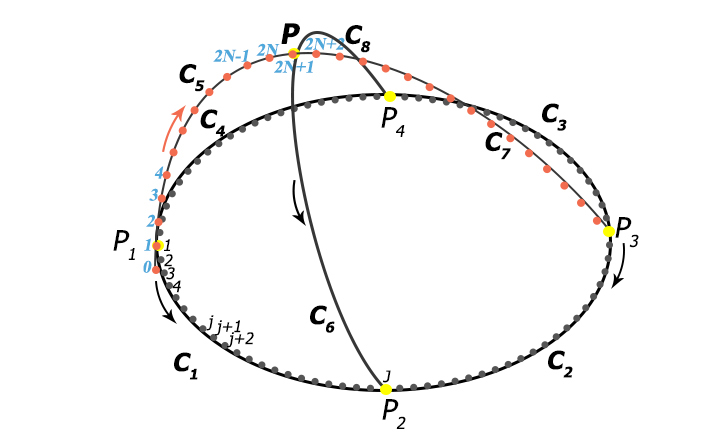
\includegraphics[width=0.7\columnwidth]{./figure/2open1close.jpeg}
	\end{center}
	\caption{Finite difference nodes for Algorithm for two open and one closed silhouette contours}
	\label{fig:2open1close}
\end{figure}\\
Since the construction algorithm for the 4 sweeping surfaces is the same, we take the sweeping surface defined by the three curves $\mathbf{c_1}$, $\mathbf{c_6}$ and $\mathbf{c_5}$ to demonstrate the construction algorithm. This algorithm will require reconstruction of the curves $\mathbf{c_5}$ and $\mathbf{c_6}$ to get additional information called sculpting forces for generating the sweeping surface.\\
In order to reconstruct the curves $\mathbf{c_5}$ and $\mathbf{c_6}$ accurately, we modify the vector-valued ordinary differential equation \eqref{ODE} by introducing a sculpting force $\mathbf{f}$ and obtain
\begin{equation}
k_b\frac{\partial^4d}{\partial u^4}-k_s\frac{\partial^2 d}{\partial u^2}=f
\label{ODEwithforce}
\end{equation}
Accordingly, the finite difference equation for the above ordinary differential equation becomes\\
\begin{equation}
\begin{split}
(6k_b+2k_sh^2)d_i+k_bd_{i-2}+k_bd_{i+2} \\
-(4k_b+k_sh^2)d_{i-1}-(4k_b+k_sh^2)d_{i+1}=\triangle u^4f_i
\end{split}
\label{odefdmwithforce}
\end{equation}
The reconstruction algorithm for the curve $\mathbf{c_6}$ is exactly same as that of the curve $\mathbf{c_5}$. Here we take the reconstruction of the curve $\mathbf{c_5}$ to demonstrate the algorithm.\\
Similar to the previous treatment, we uniformly divide the domain of the parametric variable $u$ for the curve $\mathbf{c_5(u)}$ into $2N$ equal intervals. The vector-valued first derivatives of the curves $\mathbf{c_5(u)}$ at the node 1 and $2N+1$ can be determined from the curve $\mathbf{c_5(u)}$ and indicated by $\mathbf{\mathbf{T_{5,0}}}$ and $\mathbf{T_{5,1}}$.\\
When writing the finite difference equations for the inner nodes 2, and $2N$, the node 0 beyond the boundary node 1 and the node $2N+2$ beyond the boundary node $2N+1$ will be involved. We can use the method given in Subsection \ref{ssec:num2} to determine the nodes 0 and 2N+2 from the vector-valued first derivatives $\mathbf{\mathbf{T_{5,0}}}$ and $\mathbf{T_{5,1}}$ through\\
\begin{equation}
\begin{split}
\mathbf{d_0}=\mathbf{d_2}-2\mathbf{T_{5,0}}\triangle u \\
\mathbf{d_{2N+2}}=\mathbf{d_{2N}}+2\mathbf{T_{5,1}}\triangle u
\end{split}
\label{2endsdelta}
\end{equation}\\
For each of the inner nodes 2, 3, \ldots, $2N-1$, $2N$, we can write a finite difference equation. Since the coordinate values for all the nodes on the curve $\mathbf{c_6}$ are known, we can calculate the sculpting force $\mathbf{f_i}$$(i=2,3,\ldots,2N-1,2N)$ from these equations,. We denote these sculpting forces as $\mathbf{f_{5,i}=f_i}$$(i=2,3,\ldots,2N-1,2N)$. With the same method, we can obtain the sculpting forces $\mathbf{f_{5,i}=f_i}$$(i=2,3,\ldots,2N-1,2N)$ acting on the curve $c_6$.\\
The curves $\mathbf{c_5}$ and $\mathbf{c_6}$ can be regarded as generators. The generation of the sweeping surface defined by the three curves $\mathbf{c_1}$, $\mathbf{c_6}$ and $\mathbf{c_5}$ is to sweep the generator from the curve $\mathbf{c_5}$ to the curve $\mathbf{c_6}$ along the curve $\mathbf{c_1}$ and the point $\mathbf{p}$. In order to determine the shape of the generator at different positions along the curve $\mathbf{c_1}$, we uniformly divide the curve $\mathbf{c_1}$ into $J$ equal intervals and obtain the nodes $j=1,2,3,\ldots,J-2,J-1,J$ where $j=1$ and $j=J$ are the intersecting points between the curves $\mathbf{c_5}$ and $\mathbf{c_1}$ and between $\mathbf{c_6}$ and $\mathbf{c_1}$. Then we determine the shape of the generator between the node $j(j=2,3,\ldots,J-2,J-1,J)$ and the point $\mathbf{p}$.\\
With the same treatment, we divide the domain of the parametric variable $u$ for the generator between the node $j$ and the point $\mathbf{p}$ into $2N$ equal intervals (the node $j$ on the curve $\mathbf{c_1}$ is the node 0 on the generator between the node $j$ and the point $\mathbf{p}$). When sweeping the curve $\mathbf{c_5}$ along the curve $\mathbf{c_1}$ to the curve $\mathbf{c_6}$, the sculpting force  acting at the node  of the curve is gradually changed to the sculpting force $\mathbf{f_i}$ acting at the node $i$ of the curve $\mathbf{c_6}$ . Here we use a linear interpolation to describe the gradual change and obtain the sculpting force $\mathbf{fi}$ below acting at the node $i$ of the generator between the node $j$ and the point $\mathbf{p}$\\
\begin{equation}
\centering
\mathbf{f_i}=\mathbf{f_{5,i}}+\frac{L_j}{L}(\mathbf{f_{6,i}}-\mathbf{f_{5,i}})
\label{forceinterpolate}
\end{equation}
where $L_j$ is the length from the point $\mathbf{p_1}$ to the node j and $L$ is the length from the point $\mathbf{p_1}$ to the point $\mathbf{p_2}$.
When sweeping the curve $\mathbf{c_5}$ along the curve $\mathbf{c_1}$ to the curve $\mathbf{c_6}$, the vector-valued first derivatives of the curve $\mathbf{c_5}$ at the points $\mathbf{p}$ and $\mathbf{p_1}$ are also gradually changed to the vector-valued first derivatives of the curve $\mathbf{c_6}$ at the points $\mathbf{p}$ and $\mathbf{p_2}$ . The same linear interpolation is used to describe such a gradual change and determine the vector-valued first derivatives $\mathbf{T_0}$ and $\mathbf{T_1}$ of the generator at the node $j$ and the point $\mathbf{p}$.\\
\begin{equation}
\begin{split}
\mathbf{T_0}=\mathbf{T_{5,0}}+\frac{L_j}{L}(\mathbf{T_{6,0}}-\mathbf{T_{5,0}}) \\
\mathbf{T_1}=\mathbf{T_{5,1}}+\frac{L_j}{L}(\mathbf{T_{6,1}}-\mathbf{T_{5,1}})
\end{split}
\label{tangentinterpolate}
\end{equation}
Having known the sculpting forces at all the inner nodes 2, 3, \ldots, $2N-1$, $2N$, and the coordinate values at the boundary nodes 1 and $2N+1$ and the nodes 0 and $2N+2$ beyond the boundary nodes, we can write the finite difference equations for all the inner nodes where the finite difference equations for the nodes 4, 5,\ldots, $2N-3$, $2N-2$ are the same as Equation \eqref{ODEwithforce} with the sculpting force $\mathbf{f_i}$ being calculated by Equation \eqref{forceinterpolate}\\%, and the finite difference equations for the nodes 2, 3, 2N-1, and 2N are given in Appendix D.
Solving all the finite difference equations, we obtain all the unknown constants $\mathbf{d_2}$, $\mathbf{d_3}$ , \ldots, $\mathbf{d_{2N-1}}$ and $\mathbf{d_{2N}}$ . They together with the two known points  $\mathbf{d_1}$ and  $\mathbf{p}$ are used to create the generator.\\
With the same method, we obtain all the curves of the generator at the positions $j=1,2,3,\ldots, J-2, J-1, J$. They are used to create the sweeping surface shown in Figure \ref{fig:2open1close}(b).\\
\begin{figure}[!h]
\centering
  % Fixed length
 \subcaptionbox{front\label{mouth_contour_front}}{\fbox{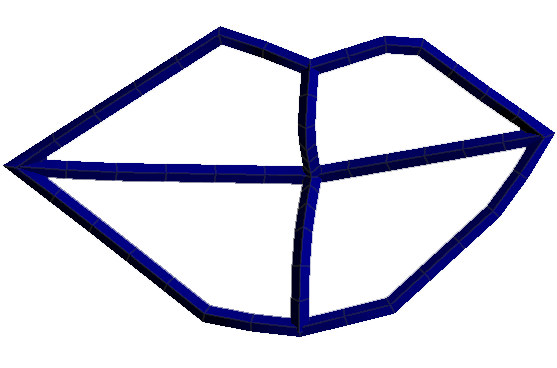
\includegraphics[height=0.5in]{./figure/mouth_contour_front.png}}}\hspace{1em}%
  \subcaptionbox{side\label{mouth_contour_side}}{\fbox{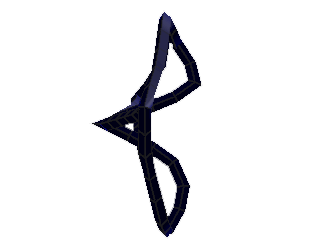
\includegraphics[height=0.5in]{./figure/mouth_contour_side.png}}}\hspace{1em}%
  \subcaptionbox{perspective\label{mouth_persp}}{\fbox{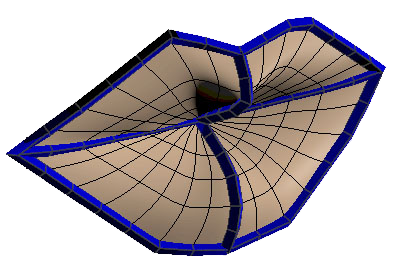
\includegraphics[height=0.5in]{./figure/mouth_contour.png}}}  
%\begin{subfigure}{0.32\linewidth}
%\centering
%\fbox{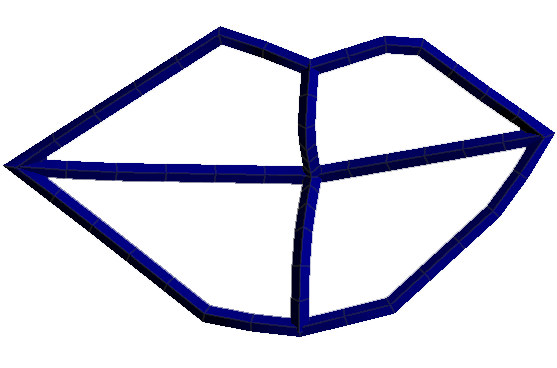
\includegraphics[height=0.5in]{./figure/mouth_contour_front.png}}\caption{front}\label{mouth_contour_front}
%\end{subfigure}
%\begin{subfigure}{0.33\linewidth}
%\centering
%\fbox{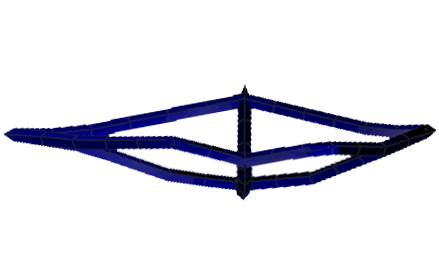
\includegraphics[height=0.5in]{./figure/mouth_contour_top.png}}\caption{top}\label{mouth_contour_top}
%\end{subfigure}
%\begin{subfigure}{0.32\linewidth}
%\centering
%\fbox{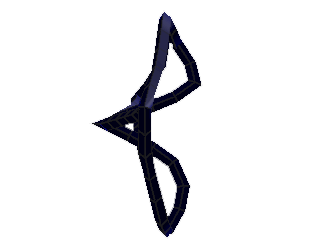
\includegraphics[height=0.5in]{./figure/mouth_contour_side.png}}\caption{side}\label{mouth_contour_side}
%\end{subfigure}
%\begin{subfigure}{0.32\linewidth}
%\centering
%\fbox{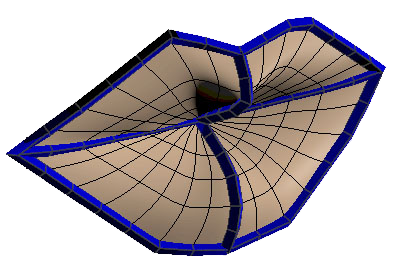
\includegraphics[height=0.5in]{./figure/mouth_contour.png}}\caption{perspective}\label{mouth_persp}
%\end{subfigure}
%\begin{subfigure}{0.45\linewidth}
%\centering
%\fbox{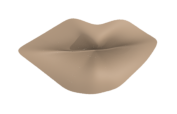
\includegraphics[height=0.5in]{./figure/mouth_mesh.png}}\caption{mesh}\label{mouth_mesh}
%\end{subfigure}
  \caption{mouth model creation from two open and one closed silhouette contours in three different view planes}
 \label{fig:mouth}
\end{figure}  \\
With the above method, we draw a closed lip contour and two open curves shown in Figure \ref{fig:mouth}\subref{fig:mouth_contour}. They divide the palm into four regions. One surface is created each of the four regions. Figure \ref{fig:mouth}\subref{fig:mouthmesh} depicts the palm model consisting of the four surfaces. \\
\begin{figure}[!h]
\centering
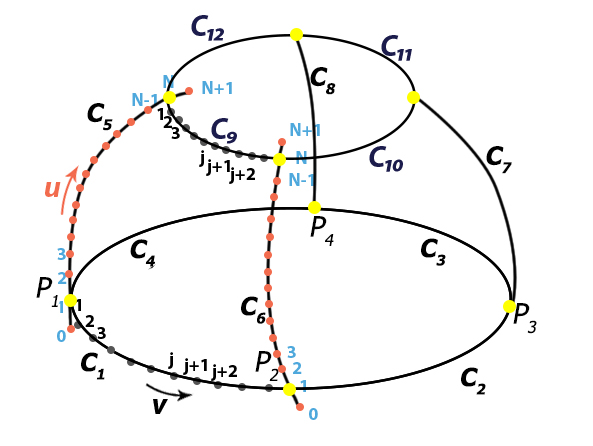
\includegraphics[width=0.7\columnwidth]{./figure/4open2close.jpg}
\label{fig:4opens2closedalgorithm}
\caption{Finite difference nodes for Algorithm for four open and two closed silhouette contours}
\end{figure} \\
The above method can be also extended to deal with the situations where the two open curves do not intersect. For such situations, the intersecting point of the two open curves becomes the upper closed curve as indicated in Figures \ref{fig:4opens2closedalgorithm}, and a sweeping surface is encircled by four curves. With this extension, we created a 3D vest model and an eye socket model depicted it in Figures \ref{fig:4opens2closed}\subref{fig:vest} and Figures \ref{fig:4opens2closed}\subref{fig:eye}, respectively. \\
\begin{figure}[!h]
  % Fixed length
\subcaptionbox{vest\label{vest}}{ 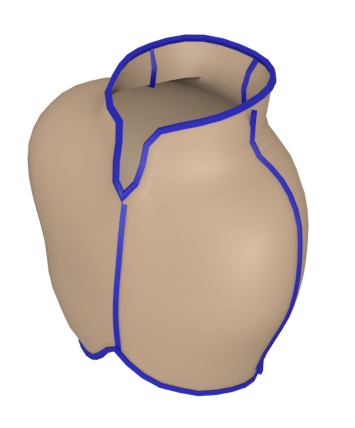
\includegraphics[height=0.1\textheight]{./figure/uppertorso.png}}\hspace{3em}%
\subcaptionbox{eye soket\label{eye}}{ 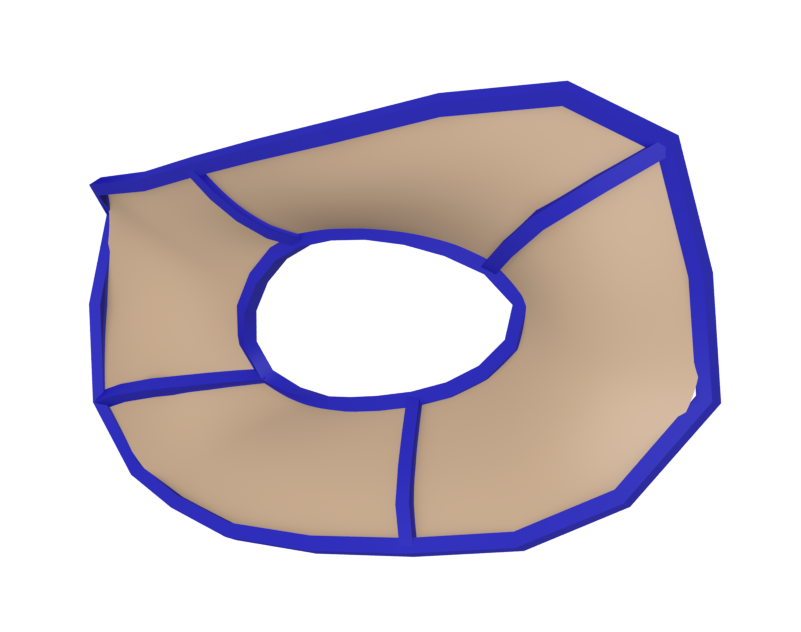
\includegraphics[height=0.1\textheight]{./figure/eye.png}}
 \caption{vest and eye socket creation from four open and two closed silhouette contours}
 \label{fig:4opens2closed}
\end{figure}  

\subsubsection{Algorithm for 4-sided open curves}
%Spline patch is a very commonly used modelling technology to create a spline surface and gained its popularity in Computer Aided Design/Manufacturing for its power to achieve shape accuracy. Usually the shape of a neighbourhood near the patches' borders is determined by the control points and can be influenced by its adjacent patches if users have set the geometric continuity of the borders. In the realm of spline patches, the problem of influencing the patch's shape near the border without change much of the rest of the patches is called mesh optimisation. A typical way of solving that problem is to formulate a geometric constraints matrix as the coefficient matrix of a homogeneous linear equation and the solution to that equation is the displacements of the control points that we are looking for\cite{zhang2016geometric}. makes the look of patch more well-defined. 
We introduce a new physic-based ODE-driven algorithm for making patch surfaces by asking them providing a virtual border a little bit far away beyond the actual border. This virtual border can be a curve from the adjacent patch, like that in the typical mesh optimisation problems where C1 continuity is required on the joint border.Taken the virtual border's positional information into the constraint matrix formation, solve this linear equation and the solution to that equation is the position of every vertex. Our algorithm enables users to refine the border areas with or without the existence of adjacent patches. In addition, compared to the typical way of solving the border continuity optimisation\cite{zhang2016geometric}, our method is computational cheaper because though both required forming a constraint matrix as a coefficient matrix of a linear equation, instead of getting the displacements of the control points and then computing the spline surface out of the modified control points, our method get the vertex positions of the final parametric surface straight away.
\begin{figure}[!h]
\centering
\includegraphics[width=0.7\columnwidth]{./figure/4open2close.jpg}
\label{fig:4-sidedopensalgorithm}
\caption{Finite difference nodes for Algorithm for four-sided open silhouette contours with arbitrary number of curves in either direction}
\end{figure} \\
As demonstrated in Figure \ref{fig:4-sidedopensalgorithm}, the sweeping surface passing through all the curves can be seen as a tweak of the closed surface in Figure \ref{4opens2closedalgorithm}. The 
encircled by the curves $\mathbf{c_1c_6c_5}$, $\mathbf{c_2c_7c_6}$, $\mathbf{c_3c_8c_7}$, and $\mathbf{c_4c_5c_8}$ respectively.\\
\begin{figure}[h]
	\begin{center}
	\includegraphics[width=0.7\columnwidth]{./figure/2open1close.jpeg}
	\end{center}
	\caption{Finite difference nodes for Algorithm for two open and one closed silhouette contours}
	\label{fig:2open1close}
\end{figure}\\
Since the construction algorithm for the 4 sweeping surfaces is the same, we take the sweeping surface defined by the three curves $\mathbf{c_1}$, $\mathbf{c_6}$ and $\mathbf{c_5}$ to demonstrate the construction algorithm. This algorithm will require reconstruction of the curves $\mathbf{c_5}$ and $\mathbf{c_6}$ to get additional information called sculpting forces for generating the sweeping surface.\\
In order to reconstruct the curves $\mathbf{c_5}$ and $\mathbf{c_6}$ accurately, we modify the vector-valued ordinary differential equation \eqref{ODE} by introducing a sculpting force $\mathbf{f}$ and obtain
\begin{equation}
k_b\frac{\partial^4d}{\partial u^4}-k_s\frac{\partial^2 d}{\partial u^2}=f
\label{ODEwithforce}
\end{equation}
Accordingly, the finite difference equation for the above ordinary differential equation becomes\\
\begin{equation}
\begin{split}
(6k_b+2k_sh^2)d_i+k_bd_{i-2}+k_bd_{i+2} \\
-(4k_b+k_sh^2)d_{i-1}-(4k_b+k_sh^2)d_{i+1}=\triangle u^4f_i
\end{split}
\label{odefdmwithforce}
\end{equation}
The reconstruction algorithm for the curve $\mathbf{c_6}$ is exactly same as that of the curve $\mathbf{c_5}$. Here we take the reconstruction of the curve $\mathbf{c_5}$ to demonstrate the algorithm.\\
Similar to the previous treatment, we uniformly divide the domain of the parametric variable $u$ for the curve $\mathbf{c_5(u)}$ into $2N$ equal intervals. The vector-valued first derivatives of the curves $\mathbf{c_5(u)}$ at the node 1 and $2N+1$ can be determined from the curve $\mathbf{c_5(u)}$ and indicated by $\mathbf{\mathbf{T_{5,0}}}$ and $\mathbf{T_{5,1}}$.\\
When writing the finite difference equations for the inner nodes 2, and $2N$, the node 0 beyond the boundary node 1 and the node $2N+2$ beyond the boundary node $2N+1$ will be involved. We can use the method given in Subsection \ref{ssec:num2} to determine the nodes 0 and 2N+2 from the vector-valued first derivatives $\mathbf{\mathbf{T_{5,0}}}$ and $\mathbf{T_{5,1}}$ through\\
\begin{equation}
\begin{split}
\mathbf{d_0}=\mathbf{d_2}-2\mathbf{T_{5,0}}\triangle u \\
\mathbf{d_{2N+2}}=\mathbf{d_{2N}}+2\mathbf{T_{5,1}}\triangle u
\end{split}
\label{2endsdelta}
\end{equation}\\
For each of the inner nodes 2, 3, \ldots, $2N-1$, $2N$, we can write a finite difference equation. Since the coordinate values for all the nodes on the curve $\mathbf{c_6}$ are known, we can calculate the sculpting force $\mathbf{f_i}$$(i=2,3,\ldots,2N-1,2N)$ from these equations,. We denote these sculpting forces as $\mathbf{f_{5,i}=f_i}$$(i=2,3,\ldots,2N-1,2N)$. With the same method, we can obtain the sculpting forces $\mathbf{f_{5,i}=f_i}$$(i=2,3,\ldots,2N-1,2N)$ acting on the curve $c_6$.\\
The curves $\mathbf{c_5}$ and $\mathbf{c_6}$ can be regarded as generators. The generation of the sweeping surface defined by the three curves $\mathbf{c_1}$, $\mathbf{c_6}$ and $\mathbf{c_5}$ is to sweep the generator from the curve $\mathbf{c_5}$ to the curve $\mathbf{c_6}$ along the curve $\mathbf{c_1}$ and the point $\mathbf{p}$. In order to determine the shape of the generator at different positions along the curve $\mathbf{c_1}$, we uniformly divide the curve $\mathbf{c_1}$ into $J$ equal intervals and obtain the nodes $j=1,2,3,\ldots,J-2,J-1,J$ where $j=1$ and $j=J$ are the intersecting points between the curves $\mathbf{c_5}$ and $\mathbf{c_1}$ and between $\mathbf{c_6}$ and $\mathbf{c_1}$. Then we determine the shape of the generator between the node $j(j=2,3,\ldots,J-2,J-1,J)$ and the point $\mathbf{p}$.\\
With the same treatment, we divide the domain of the parametric variable $u$ for the generator between the node $j$ and the point $\mathbf{p}$ into $2N$ equal intervals (the node $j$ on the curve $\mathbf{c_1}$ is the node 0 on the generator between the node $j$ and the point $\mathbf{p}$). When sweeping the curve $\mathbf{c_5}$ along the curve $\mathbf{c_1}$ to the curve $\mathbf{c_6}$, the sculpting force  acting at the node  of the curve is gradually changed to the sculpting force $\mathbf{f_i}$ acting at the node $i$ of the curve $\mathbf{c_6}$ . Here we use a linear interpolation to describe the gradual change and obtain the sculpting force $\mathbf{fi}$ below acting at the node $i$ of the generator between the node $j$ and the point $\mathbf{p}$\\
\begin{equation}
\centering
\mathbf{f_i}=\mathbf{f_{5,i}}+\frac{L_j}{L}(\mathbf{f_{6,i}}-\mathbf{f_{5,i}})
\label{forceinterpolate}
\end{equation}
where $L_j$ is the length from the point $\mathbf{p_1}$ to the node j and $L$ is the length from the point $\mathbf{p_1}$ to the point $\mathbf{p_2}$.
When sweeping the curve $\mathbf{c_5}$ along the curve $\mathbf{c_1}$ to the curve $\mathbf{c_6}$, the vector-valued first derivatives of the curve $\mathbf{c_5}$ at the points $\mathbf{p}$ and $\mathbf{p_1}$ are also gradually changed to the vector-valued first derivatives of the curve $\mathbf{c_6}$ at the points $\mathbf{p}$ and $\mathbf{p_2}$ . The same linear interpolation is used to describe such a gradual change and determine the vector-valued first derivatives $\mathbf{T_0}$ and $\mathbf{T_1}$ of the generator at the node $j$ and the point $\mathbf{p}$.\\
\begin{equation}
\begin{split}
\mathbf{T_0}=\mathbf{T_{5,0}}+\frac{L_j}{L}(\mathbf{T_{6,0}}-\mathbf{T_{5,0}}) \\
\mathbf{T_1}=\mathbf{T_{5,1}}+\frac{L_j}{L}(\mathbf{T_{6,1}}-\mathbf{T_{5,1}})
\end{split}
\label{tangentinterpolate}
\end{equation}
Having known the sculpting forces at all the inner nodes 2, 3, \ldots, $2N-1$, $2N$, and the coordinate values at the boundary nodes 1 and $2N+1$ and the nodes 0 and $2N+2$ beyond the boundary nodes, we can write the finite difference equations for all the inner nodes where the finite difference equations for the nodes 4, 5,\ldots, $2N-3$, $2N-2$ are the same as Equation \eqref{ODEwithforce} with the sculpting force $\mathbf{f_i}$ being calculated by Equation \eqref{forceinterpolate}\\%, and the finite difference equations for the nodes 2, 3, 2N-1, and 2N are given in Appendix D.
Solving all the finite difference equations, we obtain all the unknown constants $\mathbf{d_2}$, $\mathbf{d_3}$ , \ldots, $\mathbf{d_{2N-1}}$ and $\mathbf{d_{2N}}$ . They together with the two known points  $\mathbf{d_1}$ and  $\mathbf{p}$ are used to create the generator.\\
With the same method, we obtain all the curves of the generator at the positions $j=1,2,3,\ldots, J-2, J-1, J$. They are used to create the sweeping surface shown in Figure \ref{fig:2open1close}(b).\\
\begin{figure}[!h]
\centering
  % Fixed length
 \subcaptionbox{front\label{mouth_contour_front}}{\fbox{\includegraphics[height=0.5in]{./figure/mouth_contour_front.png}}}\hspace{1em}%
  \subcaptionbox{side\label{mouth_contour_side}}{\fbox{\includegraphics[height=0.5in]{./figure/mouth_contour_side.png}}}\hspace{1em}%
  \subcaptionbox{perspective\label{mouth_persp}}{\fbox{\includegraphics[height=0.5in]{./figure/mouth_contour.png}}}  
  \caption{mouth model creation from two open and one closed silhouette contours in three different view planes}
 \label{fig:mouth}
\end{figure}  \\
With the above method, we draw a closed lip contour and two open curves shown in Figure \ref{fig:mouth}\subref{fig:mouth_contour}. They divide the palm into four regions. One surface is created each of the four regions. Figure \ref{fig:mouth}\subref{fig:mouthmesh} depicts the palm model consisting of the four surfaces. \\

The above method can be also extended to deal with the situations where the two open curves do not intersect. For such situations, the intersecting point of the two open curves becomes the upper closed curve as indicated in Figures \ref{fig:4opens2closedalgorithm}, and a sweeping surface is encircled by four curves. With this extension, we created a 3D vest model and an eye socket model depicted it in Figures \ref{fig:4opens2closed}\subref{fig:vest} and Figures \ref{fig:4opens2closed}\subref{fig:eye}, respectively. \\
\begin{figure}[!h]
  % Fixed length
\subcaptionbox{vest\label{vest}}{ \includegraphics[height=0.1\textheight]{./figure/uppertorso.png}}\hspace{3em}%
\subcaptionbox{eye socket\label{eye}}{ \includegraphics[height=0.1\textheight]{./figure/eye.png}}
 \caption{vest and eye socket creation from four open and two closed silhouette contours}
 \label{fig:4opens2closed}
\end{figure}  

\subsubsection{Algorithm for two closed curves}
This algorithm is to create smooth transition surfaces between two disconnected primitives. Users can interactively draw two closed curves on two disconnect primitives or use two planes to intersect the two primitives to obtain two boundary curves of the transition surface. In order to obtain smooth transition between the two primitives and the transition surface, the tangents at the two boundary curves are obtained from the two primitives. With the two boundary curves and the tangents at the two boundary curves as the boundary conditions, the ODE-based surface blending method introduced in \cite{you2014blending} is used to create the smooth transition surface which smoothly connects two primitives together. Figure \ref{fig:blend} gives such an example.\\
\begin{figure}[!h]
\centering
 \subcaptionbox{detached primitives\label{detach}}{\includegraphics[width=0.4\linewidth]{./figure/detach.png}}
  \subcaptionbox{add transition surface\label{attached}}{\includegraphics[width=0.4\linewidth]{./figure/attached.png}}
 \caption{Creation of smooth transition surface between primitives}
 \label{fig:blend}
\end{figure}  
By adding local shapes and smooth transition surface, the base mesh shown in Figure \ref{fig:system_overview}\subref{fig:primitives_after_deformation} is changed into that depicted in Figure \ref{fig:system_overview}\subref{fig:blending_body_parts}. \\
%------------------------------------------------------------------------
\section{Conclusions and Future work}\label{conclusions_and_future_work}
Compared to traditional polygon modelling technology, our method has these advantages:
 \begin{itemize}
  \item quicker
  \item easier for beginner
  \item more precise in term of detail creation 
\end{itemize}
 
I did the experiment of deforming a toy rubber tyre. The original and deformed shapes are attached on this email. The original inner circle has a diameter of 3 cm. After the deformation, the two opposite points are moved 0.3 cm each to make the length of the major axis of the ellipse 3.6 cm.  After you complete the three tasks, you can use the ODE algorithm to calculate the deformed shape and check whether the calculated deformed shape is close to the attached deformed inner ellipse.
 
The height of the toy rubber tyre which I used is too big. If the ODE deformation can give a good approximation, it can be improved by looking for a rubber ring with a small height to do the experiment. At the present time, could you please focus on the three tasks which I talked to you today morning.
%For now in the modelling stage of our system, all our control curves are creating smooth surfaces with C2 continuity, and the result template mesh looks pleasing as it is. In our future work, we will investigate the potentials of creases in more detailed character sculpting.
%-------------------------------------------------------------------------
\section*{Acknowledgement}
%This research is supported the PDE-GIR project which has received funding from the European Union's Horizon 2020 research and innovation programme under the Marie Sklodowska-Curie grant agreement No 778035.\\
This work is supported by the funding to be detailed after the anonymous review.
%\subsection{References}

%List and number all bibliographical references in 9-point Times, single-spaced, at the end of your paper. When referenced in the text, enclose the citation number in square brackets, for example~\cite{Authors12}.  Where appropriate, include the name(s) of editors of referenced books.


%-------------------------------------------------------------------------
%\subsection{Illustrations, graphs, and photographs}

%All graphics should be centered.  Please ensure that any point you wish to make is resolvable in a printed copy of the paper.  Resize fonts in figures to match the font in the body text, and choose line widths which render effectively in print.  Many readers (and reviewers), even of an electronic copy, will choose to print your paper in order to read it.  You cannot insist that they do otherwise, and therefore must not assume that they can zoom in to see tiny details on a graphic.

%When placing figures in \LaTeX, it's almost always best to use \verb+\includegraphics+, and to specify the  figure width as a multiple of the line width as in the example below
%-------------------------------------------------------------------------

{\small
\bibliographystyle{cvm}
\bibliography{cvmbib}
}


\end{document}
